% The 2026 Nobel forecasting pipeline of the Nobel Prize repository (Author_profile): models, content and usage,
% Physiology or Medicine, Physics, Chemistry and Economic Sciences. Written from the repository files
% (READMEs, SPEC/LOG files, config files, scripts, questions, context notes, run tables) after the last announcement
% (12 October 2026). Compile with pdfLaTeX, three passes (longtable, table of contents, cross references):
%   export PATH=/software/texlive-2023/bin/x86_64-linux:$PATH
%   export TEXMFVAR=/scratch/midway3/$USER/texmf-var2023b
%   mkdir -p build && for i in 1 2 3; do pdflatex -interaction=nonstopmode -output-directory build nobel2026_pipeline.tex > build/run$i.log; done
\documentclass[11pt,a4paper]{article}
\usepackage[T1]{fontenc}
\usepackage[utf8]{inputenc}
\usepackage{lmodern}
\DeclareUnicodeCharacter{2010}{-}
\DeclareUnicodeCharacter{2011}{-}
\DeclareUnicodeCharacter{2212}{\ensuremath{-}}
\DeclareUnicodeCharacter{2264}{\ensuremath{\le}}
\DeclareUnicodeCharacter{2265}{\ensuremath{\ge}}
\DeclareUnicodeCharacter{00D7}{\ensuremath{\times}}
\DeclareUnicodeCharacter{2192}{\ensuremath{\rightarrow}}
\usepackage[margin=22mm]{geometry}
\usepackage{amsmath,amssymb}
\usepackage{booktabs,longtable,tabularx,array,multirow}
\usepackage{xcolor}
\usepackage{fvextra}
\usepackage{enumitem}
\usepackage{caption}
\usepackage{float}
\usepackage{graphicx}
\usepackage{tikz}
\usetikzlibrary{positioning,arrows.meta,fit,calc}
\usepackage{microtype}
\PassOptionsToPackage{obeyspaces,spaces}{url}   % keep (and break at) spaces in \code and \file
\usepackage[hidelinks]{hyperref}
\usepackage{xurl}
\DeclareUrlCommand\code{\urlstyle{tt}}                           % inline code, breakable
\setlength{\emergencystretch}{3em}
\setlength{\LTcapwidth}{\textwidth}
\setlist{itemsep=1pt,topsep=3pt}
\captionsetup{font=small,labelfont=bf}
\fvset{breaklines=true,breakanywhere=true,fontsize=\scriptsize,frame=single,framesep=2mm}
\newcolumntype{L}{>{\raggedright\arraybackslash}X}
\newcolumntype{P}[1]{>{\raggedright\arraybackslash}p{#1}}
\DeclareRobustCommand{\ttc}[1]{\texttt{\detokenize{#1}}}   % for headings and captions (moving arguments)
\setcounter{tocdepth}{2}
\newcommand{\file}[1]{\path{#1}}
\definecolor{boxgrey}{HTML}{F3F5F6}
\definecolor{ink}{HTML}{172F40}
\definecolor{teal}{HTML}{087F74}
\definecolor{award}{HTML}{C2410C}
\graphicspath{{../docs/nobel2026/}{../Data/Result/}{../docs/example/hinton/}}

\title{Forecasting the 2026 Nobel Prizes\\[4pt]
\large A virtual committee, bibliometric profiles and an AI forecaster\\[2pt]
\large Models, content and usage of the complete pipeline: Physiology or Medicine, Physics, Chemistry and Economic Sciences}
\author{Dawoon Jeong\\ \small Knowledge Lab, University of Chicago \quad + \quad Preseen}
\date{12 October 2026 (after the last announcement)}

\begin{document}
\maketitle

\begin{abstract}
\noindent
This document describes, in one place, the pipeline we built in September and October 2026 to forecast the four 2026
Nobel Prizes decided in Stockholm --- Physiology or Medicine, Physics, Chemistry and the Sveriges Riksbank Prize in
Economic Sciences --- and how to use it. Three components work together. A \emph{virtual committee} of language-model
personas, each run on three models from different providers (\code{claude-opus-5-5}, \code{gpt-5.5-2026-04-23},
\code{gemini-3.1-pro-preview}), nominates candidate discoveries and the people who made them; its ballots are
aggregated into the options of a multiple-choice question. A \emph{research-profile pipeline} turns every named person
into a dashboard and an agent-readable record of papers, patents, books and collaboration from the OpenAlex 2026-01
snapshot, PatentsView 2025-12-31, Reliance on Science and the \emph{Science of Science} metric tables; short
\emph{profile cards} compare each person with the field's laureates at the time of their prize. \emph{Preseen}'s AI
forecaster then gives probabilities for the options, without context (control) and with context notes (cards,
instructions, reference facts) under several conditions. For the three science prizes the options are discoveries
(12 + ``Other'', later 30 without ``Other''); for economics the forecast has two stages, first the field of economics
(14 JEL-based fields), then 30 candidate contributions nominated in the five leading fields by personas of the eleven
real 2026 committee members. The document gives the design and the rules of every stage, the models and prompts, the
files each script reads and writes, the commands to run each step, the results of every forecast next to the award, and
the lessons and known problems. Outcomes: optogenetics (Medicine) was the first named option when the cards were the
main evidence; Francis Halzen's neutrino astronomy (Physics) ranked 9th to 14th in every condition; the Chemistry award
(Kagan and Soai) was outside every list; in Economics the field (Macro) was first in both arms and one of the two
laureates, Michael Woodford, was in the second of 30 options, with Galí and Gertler instead of Robert E.~Hall.
\end{abstract}

\tableofcontents
\clearpage
%======================================================================================================================
\part{Overview}
%======================================================================================================================

\section{Purpose and how to read this document}\label{sec:purpose}

The pipeline answers one question per prize: \emph{which discovery (or contribution) will the 2026 Nobel Prize be
awarded for, and with what probability?} It was built and run between 30 September and 10 October 2026 for the four
prizes announced in Stockholm:

\begin{center}
\small
\begin{tabularx}{\textwidth}{@{}lllL@{}}
\toprule
Prize & Announcement (CDT) & Forecasts finished by & Awarded to \\
\midrule
Physiology or Medicine & Mon 5 Oct, 04:30 & Sun 4 Oct, 23:00 & Karl Deisseroth, Peter Hegemann, Georg Nagel \\
Physics & Tue 6 Oct, 04:45 & Mon 5 Oct, 23:00 & Francis Halzen \\
Chemistry & Wed 7 Oct, 04:45 & Tue 6 Oct, 23:00 & Henri B. Kagan, Kenso Soai \\
Economic Sciences & Mon 12 Oct, 04:45 & Sun 11 Oct, 23:00 & Robert E. Hall, Michael Woodford \\
\bottomrule
\end{tabularx}
\end{center}

No forecast was run after its prize had been announced. The pipeline has three components, used in every field:

\begin{enumerate}
\item a \textbf{virtual committee}: personas of the prize committee, each run on three language models, nominate
  candidates; their ballots are aggregated into the options of a forecasting question (Sections~\ref{sec:committee}
  and~\ref{sec:convergence});
\item a \textbf{data engine}: the research-profile pipeline that turns a name into a dashboard and an agent-readable
  record of a career, and the \emph{profile cards} built from it (Sections~\ref{sec:profiles} and~\ref{sec:cards});
\item an \textbf{AI forecaster}: Preseen's forecasting system answers the question, once without context
  (\emph{control}) and once or more with context notes (\emph{conditions}); the forecasts are compared with each other,
  with the run-to-run noise and, after the announcement, with the award (Sections~\ref{sec:preseen}--\ref{sec:analysis}).
\end{enumerate}

\noindent The economics prize uses the same three components in a different arrangement: the forecaster first predicts
the \emph{field} of economics, and a virtual committee of personas of the eleven \emph{real} 2026 committee members then
nominates candidates in the leading fields (Part~\ref{part:econ}).

\paragraph{Parts.} Part~I is the overview (architecture, timeline, models and services). Part~II describes the
components of the science pipeline (Medicine, Physics, Chemistry) with their rules. Part~III is the economics pipeline.
Part~IV gives the results of every forecast next to the award and what we learned. Part~V is the user manual:
environment, keys, step-by-step recipes with the exact commands, file formats, the repository layout, costs and the
traps we met. Paths are relative to the repository root \file{/project/jevans/Dawoon/Nobel Prize/} unless they start
with a slash.

\paragraph{Repository.} The folder is the git repository \code{Dawoon-Jeong0523/Author_profile} on GitHub (remote
\code{git@github-account:Dawoon-Jeong0523/Author_profile.git}). Work happens on branch \code{preseen-nobel-2026} and is
merged into \code{main}, whose \file{README.md} is the public front page and whose root \file{index.html} is the public
dashboard of the 1--2 October Medicine, Physics and Chemistry conditions
(\url{https://dawoon-jeong0523.github.io/Author_profile/}). Code, notebooks (without outputs), small tables, context
notes, questions and figures are versioned; parquet files, profile outputs, caches, raw model responses and Preseen
client state are not (Section~\ref{sec:versioned}).

\section{Architecture}\label{sec:architecture}

\begin{figure}[H]
\centering
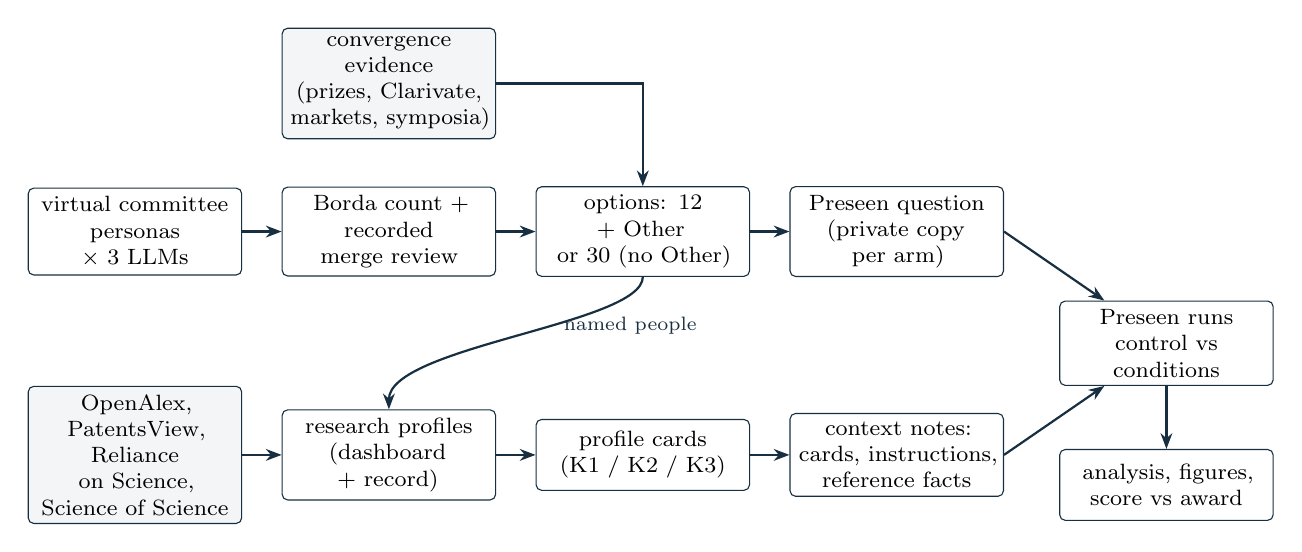
\begin{tikzpicture}[
  box/.style={draw=ink, rounded corners=2pt, align=center, font=\footnotesize, inner sep=3pt, minimum height=9mm, text width=25mm},
  data/.style={box, fill=boxgrey},
  arr/.style={-{Stealth[length=2mm]}, ink, thick},
  node distance=6mm and 5mm]
\node[box] (vc) {virtual committee\\ personas $\times$ 3 LLMs};
\node[box, right=of vc] (agg) {Borda count +\\ recorded merge review};
\node[box, right=of agg] (opt) {options: 12 + Other\\ or 30 (no Other)};
\node[data, above=of agg] (conv) {convergence evidence\\ (prizes, Clarivate,\\ markets, symposia)};
\node[box, right=of opt] (q) {Preseen question\\ (private copy per arm)};
\node[data, below=14mm of vc] (src) {OpenAlex, PatentsView,\\ Reliance on Science,\\ Science of Science};
\node[box, right=of src] (prof) {research profiles\\ (dashboard + record)};
\node[box, right=of prof] (cards) {profile cards\\ (K1 / K2 / K3)};
\node[box, right=of cards] (notes) {context notes:\\ cards, instructions,\\ reference facts};
\node[box, anchor=west] (runs) at ($(q.east)!0.5!(notes.east)+(7mm,0)$) {Preseen runs\\ control vs conditions};
\node[box, below=8mm of runs] (score) {analysis, figures,\\ score vs award};
\draw[arr] (vc) -- (agg);
\draw[arr] (agg) -- (opt);
\draw[arr] (conv) -| (opt);
\draw[arr] (opt) -- (q);
\draw[arr] (opt.south) .. controls +(0,-6mm) and +(0,8mm) .. node[font=\scriptsize, right, pos=0.4]{named people} (prof.north);
\draw[arr] (src) -- (prof);
\draw[arr] (prof) -- (cards);
\draw[arr] (cards) -- (notes);
\draw[arr] (notes.east) -- (runs);
\draw[arr] (q.east) -- (runs);
\draw[arr] (runs) -- (score);
\end{tikzpicture}
\caption{The science pipeline (Physiology or Medicine, Physics, Chemistry). Grey boxes are external data.}
\label{fig:arch}
\end{figure}

\begin{figure}[H]
\centering
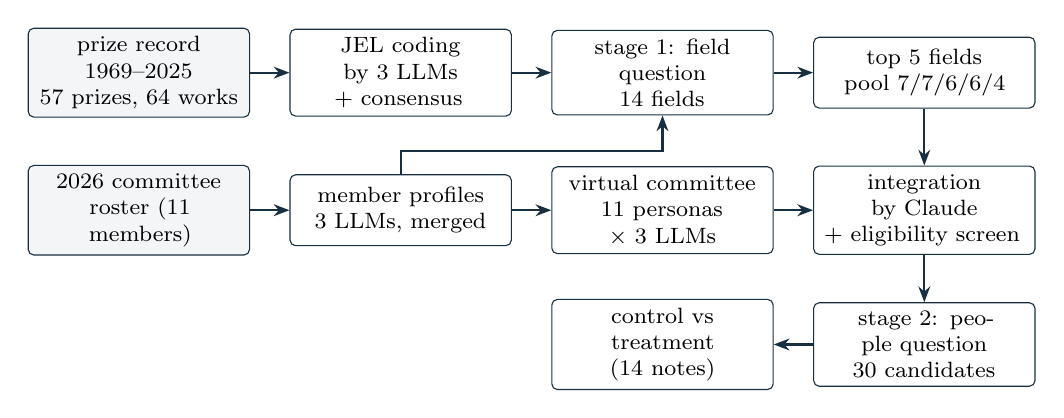
\begin{tikzpicture}[
  box/.style={draw=ink, rounded corners=2pt, align=center, font=\footnotesize, inner sep=3pt, minimum height=9mm, text width=26mm},
  data/.style={box, fill=boxgrey},
  arr/.style={-{Stealth[length=2mm]}, ink, thick},
  node distance=6mm and 5mm]
\node[data] (rec) {prize record 1969--2025\\ 57 prizes, 64 works};
\node[box, right=of rec] (jel) {JEL coding by 3 LLMs\\ + consensus};
\node[box, right=of jel] (fq) {stage 1: field question\\ 14 fields};
\node[box, right=of fq] (top) {top 5 fields\\ pool 7/7/6/6/4};
\node[data, below=of rec] (rost) {2026 committee\\ roster (11 members)};
\node[box, right=of rost] (prof) {member profiles\\ 3 LLMs, merged};
\node[box, right=of prof] (vc) {virtual committee\\ 11 personas $\times$ 3 LLMs};
\node[box, right=of vc] (int) {integration by Claude\\ + eligibility screen};
\node[box, below=of int] (pq) {stage 2: people question\\ 30 candidates};
\node[box, left=of pq] (arms) {control vs treatment\\ (14 notes)};
\draw[arr] (rec) -- (jel);
\draw[arr] (jel) -- (fq);
\draw[arr] (fq) -- (top);
\draw[arr] (rost) -- (prof);
\draw[arr] (prof) -- (vc);
\draw[arr] (prof.north) -- ++(0,3mm) -| (fq.south);
\draw[arr] (top) -- (int.north);
\draw[arr] (vc) -- (int);
\draw[arr] (int) -- (pq);
\draw[arr] (pq) -- (arms);
\end{tikzpicture}
\caption{The economics pipeline: the field first, then candidates within the leading fields (Part~\ref{part:econ}).}
\label{fig:arch-econ}
\end{figure}

\begin{table}[htbp]
\small
\begin{tabularx}{\textwidth}{@{}P{30mm}P{40mm}LP{28mm}@{}}
\toprule
Component & Folder & What it does & Models / services \\
\midrule
Research profiles & \file{pipeline/}, \file{notebook/}, \file{jobs/} & name $\rightarrow$ OpenAlex author id $\rightarrow$ Slurm job $\rightarrow$ dashboard (HTML) and record (Markdown) of papers, patents, books, networks & local data; OpenAlex API for author search and titles \\
Virtual committee, 12 + Other & \file{experiment/preseen/} & specialty personas of the 2026 committees nominate discoveries; Borda + merge review; living check; question; cards; Preseen runs; analysis; dashboard & Claude, GPT, Gemini; Wikidata; Preseen \\
Conditions on the cards & \file{experiment/preseen_cards_main/}, \file{preseen_cards_balanced/} & the same question with instructions on how to use the cards & Preseen \\
30-option lists & \file{experiment/convergence_2026/}, \file{convergence_2026_v2/} & committee options + external evidence as extra voters; v2 lineups; age-25 cards; patents tied to the discovery & Claude (patent and work picks); Wikidata \\
Physics and Chemistry runs & \file{experiment/preseen_*_v2/}, \file{preseen_chem30_main/}, \file{preseen_generated30/} & 12-, 30- and 5-option physics questions; five chemistry conditions; Preseen-drafted option list & Preseen \\
Economics & \file{Econ/} & prize record, committee profiles, JEL coding, field question, laureate ages, member-persona committee, integration, people question & Claude, GPT, Gemini; Preseen; Wikidata; Nobel Prize API \\
Results and figures & \file{Data/Result/}, \file{docs/nobel2026/} & forecast tables, Preseen reports (PDF), README figures & --- \\
Handoff & \file{handoff/} & context and forecasts of the four 1--2 October conditions, kept apart, for Preseen & --- \\
\bottomrule
\end{tabularx}
\caption{Components and where they live.}
\label{tab:components}
\end{table}

\section{Timeline}\label{sec:timeline}

\begin{longtable}{@{}P{22mm}P{139mm}@{}}
\toprule
Date (2026) & Work \\
\midrule
\endhead
30 Sep & Research-profile pipeline: \file{notebook/author_profile.ipynb}, \file{notebook/np_common.py}, dashboards; PrizeAtlas crawl; batch of all 656 OpenAlex ids of the 1901--2025 science laureates (2 h 15 min); laureate aggregate notebook. \\
1 Oct & Name pipeline \file{pipeline/profile_person.py}; git repository. Preseen context experiment (\file{experiment/preseen/}): virtual committees of the three science prizes (66 persona $\times$ model cells, all valid, \$7.12), 12 discoveries + Other per field, living check, 98 profile cards, control and ``cards as context'' questions, 21 runs (4 control + 3 treat per field). \\
2 Oct & ``Cards as the main evidence'' and ``cards as one main source'' conditions, one run per field each, plus a same-day control; combined public dashboard of the four conditions. \\
3 Oct & Inventor linking refined (\code{np_common.link_inventors}); profiles and cards rebuilt (\file{cards_v2/}); handoff of contexts and forecasts for Preseen. \\
5 Oct & \textbf{Medicine awarded.} Physics: 30-option lists from committee + convergence evidence; cards for 68 new people; age-25 cards; runs with 12, 30 and 5 options (control and main evidence). \\
6 Oct & \textbf{Physics awarded.} v2 lineup rule; cards for 32 new people; patent section of the chemistry cards; Preseen-drafted list of 30; chemistry runs: cards as the main evidence (three versions), demographic, cards as one main source, cards as context, control. \\
7 Oct & \textbf{Chemistry awarded}, outside every list; README and figures with the award; sleeping-beauty check of the awarded papers. \\
9 Oct & Economics (\file{Econ/}): prize record 1969--2025, profiles of the 11 committee members (\$4.66), JEL coding of the 64 prize works (\$1.52), field analysis. \\
10 Oct & Economics: field question (two experiments $\times$ control and treatment), laureate ages, virtual committee of member personas (33 cells, \$8.30) and integration (\$2.33), eligibility screen, people question (control and treatment); pushed to GitHub. \\
12 Oct & \textbf{Economics awarded}; READMEs and figures with the award; this document. \\
\bottomrule
\caption{Timeline. Details per step are in the \ttc{LOG.md} files of the experiment folders and in \ttc{Econ/NOTES.md}.}
\label{tab:timeline}
\end{longtable}

\section{Models and external services}\label{sec:models}

\subsection{Language models}

Three models from three providers, chosen on 1 October and kept fixed for every LLM step of all four prizes:

\begin{center}
\small
\begin{tabularx}{\textwidth}{@{}lllL@{}}
\toprule
Letter & Provider & Model id & API used (plain HTTPS with \code{requests}) \\
\midrule
A & Anthropic & \code{claude-opus-5-5} & \code{/v1/messages}, JSON schema through \code{output_config.format} \\
O & OpenAI & \code{gpt-5.5-2026-04-23} & \code{/v1/responses}, strict \code{json_schema}, \code{store=false} \\
G & Google & \code{gemini-3.1-pro-preview} & \code{generateContent} with \code{responseJsonSchema} \\
\bottomrule
\end{tabularx}
\end{center}

\noindent The same system and user text go to every provider. No tools, web search, grounding, sampling, reasoning-effort
or fallback parameters are sent, so each provider runs with its defaults; the output cap is 32,000 tokens. The reported
model string of every response is recorded and equalled the requested id. Calls are made by
\file{experiment/preseen/llm_providers.py} (science) and \file{Econ/llm_providers.py} (economics, a copy with the same
conventions). Every call is logged with its tokens and cost.

\begin{table}[htbp]
\small
\begin{tabularx}{\textwidth}{@{}P{48mm}lL@{}}
\toprule
Step & Models & Role \\
\midrule
Science committee ballots (1 Oct) & A, O, G & 22 specialty personas (6 / 8 / 8) $\times$ 3 models; up to five ranked nominations each \\
Defining works of age-25 cards, patents tied to a discovery (5--6 Oct) & Claude & choose the works or patents of a person most tied to the option's discovery \\
Committee member profiles (Econ, 9 Oct) & A, O, G; merge by A & each model describes each member from its own knowledge; Claude merges the three \\
JEL coding of the prize works (Econ, 9 Oct) & A, O, G & primary and secondary JEL codes of each of the 64 works; consensus computed locally \\
Econ committee ballots (10 Oct) & A, O, G & 11 member personas $\times$ 3 models; up to five nominations in each of five fields \\
Integration of the Econ nominations (10 Oct) & A & groups the 165 nominations of a field into distinct candidates; scores are computed locally \\
Reasoning summaries, write-ups of the record & Claude & labelled as LLM-written wherever they appear \\
\bottomrule
\end{tabularx}
\caption{Where language models enter the pipeline. Scores, aggregation, eligibility and every number in the context notes are computed in code.}
\end{table}

\subsection{Preseen}\label{sec:preseen-service}

Preseen (\url{https://preseen.com}) is an AI forecasting system with a public API. The objects we use:

\begin{itemize}
\item \textbf{Question}: a private multiple-choice question with title, description, resolution criteria, fine print and
  options (\code{options_are_mutually_exclusive}, \code{options_are_comprehensive}). One identical question is created
  per arm, because context notes attach to a question and apply to all its later runs.
\item \textbf{Context note}: a text attached to a question with a \emph{treatment}. \code{consider} makes the note one
  input among many; \code{assume_true} makes it a premise. In our runs \code{assume_true} instructions moved forecasts a
  great deal while \code{consider}-only cards barely did (Section~\ref{sec:res-science}), so instructions and
  reference facts are attached as \code{assume_true} and person cards as \code{consider}.
\item \textbf{Run (task)}: a forecast of the question. A run takes 25--55 minutes, searches the web itself, combines
  four subforecasts into the final forecast (\code{forecast.forecast_data.payload.probabilities}) and returns a
  write-up with sources. Preseen can also export a report (PDF), which we keep for the main runs.
\end{itemize}

\noindent The client (\file{experiment/preseen/nobel_preseen_exp.py}, copied into each run folder and into
\file{Econ/04_field_forecast/}) keeps its state in \code{$EXP_DIR/state.json}, sends an Idempotency-Key with every POST
(re-running a command never duplicates a question, note or run) and never uses watches, schedules, re-forecasts or
\code{accept-context}. Its commands are listed in Section~\ref{sec:client}.

\subsection{Data sources and lookups}

\begin{center}
\small
\begin{tabularx}{\textwidth}{@{}lL@{}}
\toprule
Source & Used for \\
\midrule
OpenAlex 2026-01 snapshot (local) and API & works, authors, institutions, co-authors; live author search; titles of works missing from the snapshot \\
PatentsView 2025-12-31 (local) & US utility patents, inventors, assignees, locations, pre-grant publications \\
Reliance on Science (Marx \& Fuegi) & patent $\rightarrow$ paper citations \\
\emph{Science of Science} metric tables (local) & citations, disruption, Foundation / Extension / Generalization, book citations, cohort percentiles \\
PrizeAtlas, Li et al.\ (2019), SciSciNet laureate links & laureates 1901--2025 with OpenAlex ids, prize papers, prize years \\
nobelprize.org list page, Nobel Prize API 2.1 & economics prize record 1969--2025 and the 2026 award \\
Wikidata (and the web for flagged cases) & living check of every named person, years of birth \\
ORCID public API & identity checks in name resolution \\
\code{Data/convergence_2026.csv} & person-level external evidence (Clarivate, prediction markets, recent prizes, Nobel symposia) for the 30-option lists \\
Dolton and Tol (2026), arXiv:2603.20767v1 & the 14 JEL-based fields of economics and field-level evidence \\
\bottomrule
\end{tabularx}
\end{center}
%======================================================================================================================
\part{The science pipeline: components}\label{part:science}
%======================================================================================================================

\section{The data engine: research profiles}\label{sec:profiles}

Every person named in a science option gets a research profile. The profile pipeline works for anybody with an
OpenAlex author record; it was first run on all 656 OpenAlex ids of the PrizeAtlas laureates in Physics, Chemistry and
Physiology or Medicine 1901--2025. Its full documentation is \file{docs/author_profiles.md}; this section summarizes
what the forecasts rely on.

\subsection{From a name to a profile}

\begin{enumerate}
\item \textbf{Candidates} (\code{np_common.find_author_candidates}): the snapshot's authors table
  (\file{cache/openalex_authors.parquet}) plus the live OpenAlex author search, in tiers: \code{display} (the display
  name agrees with the query: same surname, first name equal or an initial, no conflicting middle initial),
  \code{alias} (only an alternative name agrees; never chosen automatically), \code{orcid} and \code{prizeatlas}.
\item \textbf{Choice} (\code{pick_author}): an ORCID match decides; else the laureate's PrizeAtlas id; else the only
  display-name candidate at \code{--affiliation}; else the most cited display-name candidate if it has at least
  \code{--dominance} (default 3) times the citations of the next one; else the candidate table is printed and the run
  stops with exit status 2 for a \code{--pick}. A name shared by several laureates is never chosen by citations alone.
\item \textbf{Fragments} (\code{same_person_fragments}): candidates with the same display name, at least two works, a
  shared institution word and no different ORCID are added (OpenAlex splits prolific people).
\item \textbf{Author id check} (notebook section 0b): ids with fewer than five works in the snapshot (often ids created
  after January 2026) are resolved by ORCID, the Li et al.\ laureate bridge or name.
\item \textbf{Works}: every (work, affiliation) row of the ids in the authorship table of the 2026-01 snapshot (1.0
  billion rows), then every author of those works (co-authors). An optional work list (\code{--works-file},
  \code{NP_WORKS_FILE}) restricts the profile to given works when OpenAlex has merged namesakes into one record.
\item \textbf{Patents} --- inventor linking (\code{np_common.link_inventors}): candidates from the pqrs author--inventor
  crosswalk (PatentsView 2023-03-30 ids, translated to the 2025-12-31 release) and from a PatentsView name search; each
  candidate's patents are clustered by shared co-inventors and assignees and a cluster is linked on evidence from the
  author's own record --- \emph{strong}: a co-inventor who is a co-author with a rare name, a citation of a rarely cited
  work of the author, a small assignee that names a major affiliation; \emph{moderate}: a co-author co-inventor with a
  common name, a citation of a widely cited work, an assignee naming an affiliation, the pqrs link; \emph{conflict}:
  inventor countries outside the affiliation countries, grant years far from the publication years. Common names need
  evidence on at least 10\,\% of a cluster; patents of a selected id that belong to a namesake are left out and listed
  with the reason.
\item \textbf{Metrics}: the \emph{Science of Science} tables for papers and patents, each turned into a cohort
  percentile from shared population tables; books (OpenAlex works of type book, book chapter, book section or
  reference entry) that cite the works; Reliance on Science links from US patents and pre-grant publications.
\item \textbf{Outputs}: the dashboard, the record and the per-person folder (below).
\end{enumerate}

\subsection{Measures}

\begin{itemize}
\item \textbf{Percentile}: mid-rank share of the cohort below the document (ties split evenly). Works are compared
  with the OpenAlex works of the same publication year $\times$ first field; patents with the US utility patents of
  the same grant year $\times$ CPC section. ``Top 10\,\% / 1\,\%'' = percentile $\geq 0.90 / 0.99$.
\item \textbf{Impact}: citations in the first 5 (or 10) years; for patents citations from granted patents and pre-grant
  publications.
\item \textbf{Disruption (CD, 5 years)}: whether the papers citing a document within five years also cite its
  references. A reference-less document has CD $=1$ by construction; it is blanked, and cohort percentiles are taken
  among documents with references (\file{cache/cd_rpctl_*.parquet}).
\item \textbf{Foundation / Extension / Generalization} (5 years): the shares of citing documents that build on the
  document itself, extend it together with its references, or generalize over them (Fang and Evans, arXiv:2510.03240).
\item \textbf{Textbook reach}: citations from books; ``cited by at least \code{BOOK_MIN} (3) books''.
\item \textbf{Window}: works published and patents granted up to \code{YEAR_MAX} (2021); window measures need the window
  closed by 2026. Headline statistics use research works (article, review, letter).
\end{itemize}

\subsection{Outputs}

\begin{itemize}
\item \textbf{Dashboard} \file{output/dashboard/<year>_<field>_<name>_<author id>.html}: one standalone HTML page
  (plotly embedded, about 5\,MB): header tiles; every document against its cohort; cumulative output; percentiles and
  citations per year; books; patent citations; co-authorship, co-invention, combined, institution and assignee networks;
  the top documents.
\item \textbf{Record} \file{output/record/<same name>.md}: Markdown for agents with a YAML header (\code{record_type},
  \code{schema_version} 2, \code{query}, \code{person}, \code{nobel}, \code{window}, \code{dashboard}, \ldots) and the
  numbers behind every dashboard block. Profile cards and the handoff records are built from the per-person tables.
\item \textbf{Per-person folder} \file{output/<author id>/}: \code{papers_metrics.parquet/.csv},
  \code{patents_metrics.parquet/.csv}, \code{percentile_summary.csv}, \code{inventor_link_candidates.csv},
  \code{inventor_link_patents.csv}, network tables and GraphML, figures, \code{manifest.json}, \code{profile_summary.json}
  and a \code{_cache/} of per-person scans.
\end{itemize}

\begin{figure}[htbp]
\centering
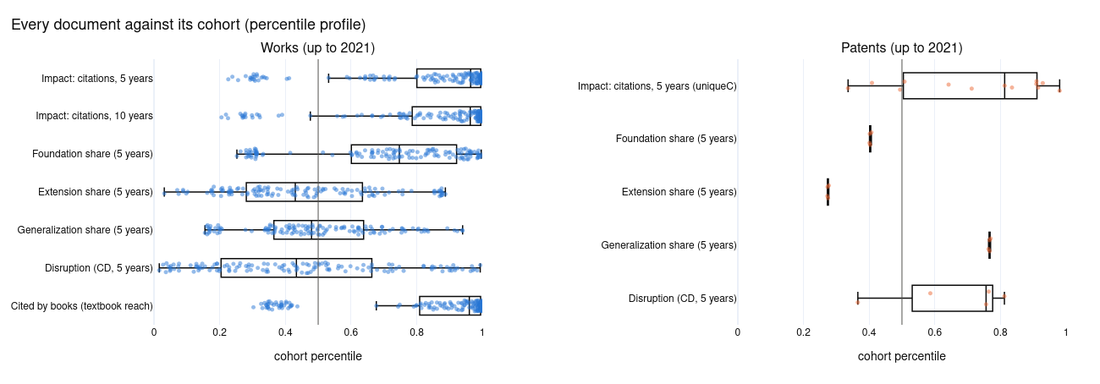
\includegraphics[width=0.48\textwidth]{percentile_profile.png}\hfill
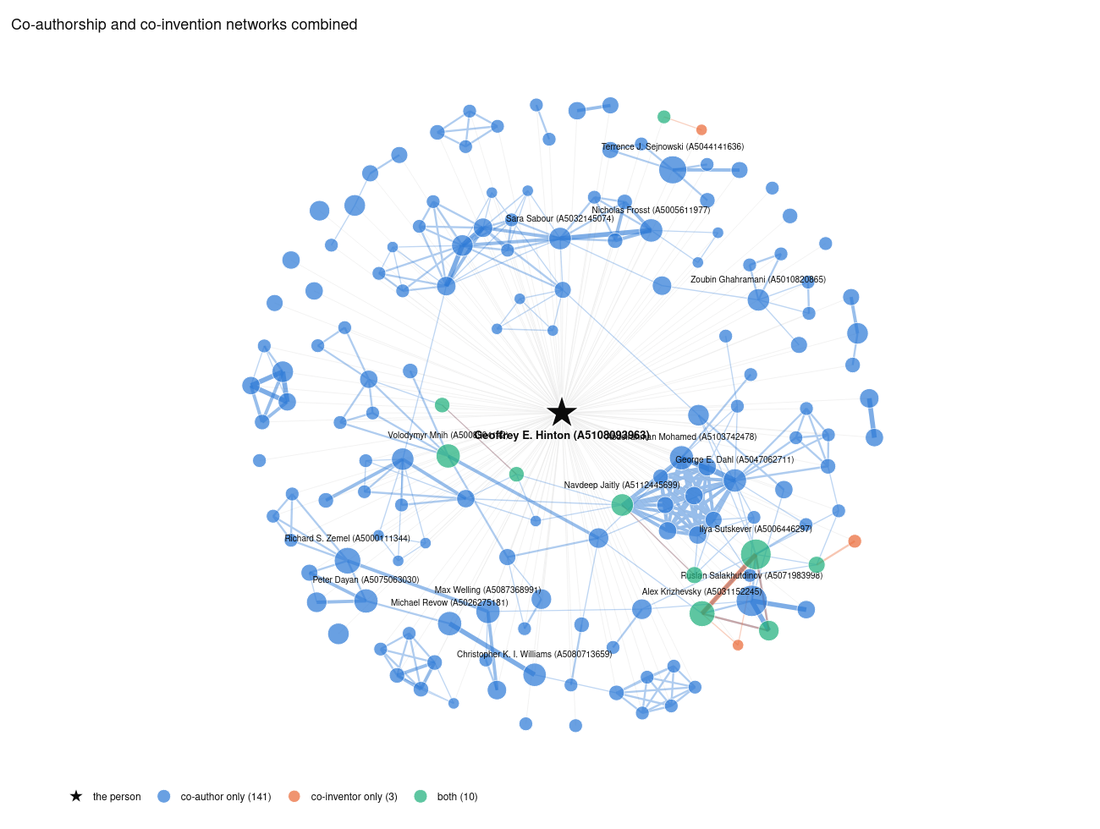
\includegraphics[width=0.48\textwidth]{combined_network.png}
\caption{Two blocks of the example dashboard (Geoffrey Hinton): every document against its cohort (left) and the
combined co-authorship / co-invention network (right). From \ttc{docs/example/hinton/}.}
\end{figure}

\subsection{Running it}

The notebook is \file{notebook/author_profile.ipynb} on the shared module \file{notebook/np_common.py}; the name
pipeline \file{pipeline/profile_person.py} resolves a name on the login node (about 30 seconds; it reads a 6\,GB
parquet) and submits a Slurm job (8 cores, 64\,GB, 1--5 minutes per person once the shared caches exist). Commands and
options are in Section~\ref{sec:use-profiles}. Notebook parameters come from the first code cell or from environment
variables (\code{NP_AUTHOR_ID}, \code{NP_EXTRA_AUTHOR_IDS}, \code{NP_WORKS_FILE}, \code{NP_YEAR_MAX},
\code{NP_ID_CHECK}, \code{NP_NAME_SEARCH}, \code{NP_VERIFY_PQRS}, \code{NP_PATENT_FILTER}, \code{NP_FETCH_TITLES},
\code{NP_TITLES_TABLE}, \code{NP_NOBEL_LOOKUP}, \code{NP_PRIZE_YEAR}, \code{NP_PRIZE_FIELD}, \code{NP_QUERY},
\code{NP_RESOLUTION}; Table~\ref{tab:np-env}).

\subsection{Known data problems that reach the cards}\label{sec:profile-caveats}

\begin{itemize}
\item About a quarter of the works of an OpenAlex author record are missing from the 2026-01 works table and carry no
  metrics (they keep patent-citation counts; titles come from the API).
\item OpenAlex merges namesakes into one author record (Jun Ye, Fei-Fei Li, James A.\ Evans) and splits prolific
  people; merged records bring a namesake's early papers (Shankar Balasubramanian's record has works from 1958) and
  their patents look linked. The age-25 cards (Section~\ref{sec:cards}) and work lists address part of this.
\item PatentsView lumps frequent names into few inventor ids (Hao Yan: one id with 117 patents of several people);
  Nam-Gyu Park's card counted 13 namesake patents (nuclear fuel assemblies); Shuji Nakamura's PrizeAtlas OpenAlex id is
  a namesake's record.
\item Percentile cohorts include every OpenAlex document type, so research works sit slightly above 0.5 on average.
  Patent cohorts 1976--1979 have inflated disruption (left-censored reference graph).
\end{itemize}
\section{The virtual committee of the science prizes}\label{sec:committee}

\file{experiment/preseen/} (protocol \file{SPEC.md}, step log \file{LOG.md}, configuration \file{config.yaml}).

\subsection{Personas and cells}

Each persona is ``a senior member of the Nobel Committee for \{prize\} whose own expertise is \{specialty\}'' ---
the specialties of the real 2026 committees, without names, without impersonation and without opinions attributed to
real people:

\begin{center}
\small
\begin{tabularx}{\textwidth}{@{}lL@{}}
\toprule
Prize & Personas \\
\midrule
Physiology or Medicine (6) & neurology; molecular systems biology; neuroscience; molecular genetics; experimental rheumatology (immunology, autoimmunity); molecular developmental biology \\
Physics (8) & astroparticle physics; theoretical magnetism; applied and theoretical quantum physics; atomic physics; general physics; theoretical physics; complex systems; experimental physics, microscopy and microanalysis \\
Chemistry (8) & nanophysics; medical biochemistry; organic chemistry; physical chemistry; inorganic and structural chemistry; molecular physics; biochemistry; theoretical chemistry \\
\bottomrule
\end{tabularx}
\end{center}

\noindent Every persona runs on all three models (a crossed persona $\times$ model design, one replicate,
\code{R_c: 1}): 18 + 24 + 24 = 66 ballots. If a provider is down the crossed structure is kept; a model is never swapped
within a field.

\subsection{Prompt}

\textbf{System:} ``You are \{persona\}. Like the real committee, which calls on expert advisers for areas outside its
members' own fields, you use your own expertise as a lens but consider discoveries from the whole of \{field\}.''
\textbf{User}, in order: the date context (``It is late September 2026; the 2026 prize has not been announced.''); the
rules that matter (the wording of Nobel's will --- ``the most important discovery'', ``discovery or invention'',
``chemical discovery or improvement''; at most three people, never posthumous, every person named must be living; a
prize may be divided between two discoveries); the field's prizes 2000--2025 with official motivations and laureates
from PrizeAtlas, with ``do not nominate them again''; the task --- up to five ranked discoveries, each with
\code{rank}, \code{discovery} (one line in the style of an official motivation), \code{people} (1--3 living people
with name and affiliation), \code{key_papers} ($\leq 3$, only if known) and \code{rationale} ($\leq 2$ sentences); one
JSON object only. \code{committee.py prompt --field medicine --persona 0} prints the exact text.

\subsection{Validation}

Structure and types are hard errors; count limits (more than five nominations, people outside 1--3, more than three
papers, more than two sentences) are warnings. Ranks are renumbered by stated rank, then position; ranks above five
earn no points. An invalid ballot is asked once more (\code{json_retries: 1}); a cell that still fails is recorded as
missing and never re-asked silently. Transient HTTP errors (408, 429, 5xx, 529) are retried after 15, 60 and 180
seconds; a 429 that reports a zero quota is not. An existing raw file is never re-asked without \code{--force}. All 66
cells were valid at the first attempt (1 October 14:17--14:36 CDT, \$7.12).

\subsection{Aggregation: model-balanced Borda}

Rank $r$ earns $6-r$ points (\code{borda_points: [5,4,3,2,1]}). Each model's points are divided by its number of valid
ballots and summed over models,
\[
  S_j \;=\; \sum_{m\in\{A,O,G\}} \frac{P_{m,j}}{B_m},
\]
so every model has the same total weight whatever its number of valid ballots. Options are sorted by $S_j$, then the
number of models, then the number of nominations, then the first nomination id; the top $K=12$ with $S_j>0$ become the
named options and ``Other'' is appended.

\paragraph{Merging.} Nominations that share a person are linked automatically (union--find). The person key is first
initial + surname with accents folded and titles removed; a key with two different middle initials is split (Charles
H.\ vs Charles L.\ Bennett). A recorded review \file{committee/<field>/merges.yaml} applies three rules: an umbrella
nomination that chains two distinct discoveries becomes an option of its own; discoveries linked only through one
shared person are split; wording taken from an outlier is replaced by the majority wording. Its keys are \code{split},
\code{merge}, \code{aliases}, \code{wording_from}, \code{people}, \code{deceased}, \code{person_notes}; each entry has a
\code{reason}; unknown ids stop the script.

\begin{center}
\small
\begin{tabular}{@{}lrrrrrrrr@{}}
\toprule
Prize & Ballots & Nominations & Options & Splits & Aliases & Wording & People (ties) & Deceased \\
\midrule
Medicine & 18 & 90 & 22 & 2 & 0 & 0 & 1 & 2 \\
Physics & 24 & 120 & 21 & 2 & 2 & 1 & 0 & 1 \\
Chemistry & 24 & 120 & 28 & 4 & 2 & 2 & 2 & 0 \\
\bottomrule
\end{tabular}
\end{center}

\paragraph{Wording and people (lineup rule v1).} The option text is the \code{wording_from} nomination if one is
named, else the member nomination with the most normalized points. People are ranked by summed normalized points over
all merged nominations (ties: number of nominations, then alphabetically); the spelling and affiliation shown are the
most frequent forms; deceased people move to the end; the top three are shown:
``\textless discovery\textgreater\ --- Name A, Name B, Name C''. (This rule put Karle and Kurahashi Neilson next to
Halzen; the v2 rule of Section~\ref{sec:convergence} shows the lineup one nomination actually wrote.)

\paragraph{Diagnostics} (\file{committee/<field>/review.md}): ballots; the candidate list; flags (deceased or replaced
person, Nobel laureate among the named, resemblance to a 2000--2025 motivation by word Jaccard $\geq 0.35$, a tie for
the last shown person, more than three people named, the same person in two options); automatic and manual merges;
``possibly the same discovery, not merged'' (Jaccard $\geq 0.4$); per-model top-12 lists and their Jaccard overlap;
cross-model consensus and single-model options; leave-one-out stability (drop a persona or a model). Outputs:
\file{candidates.json} (field, models, valid ballots per model, normalization, options), \file{clusters.json},
\file{review.md}.

\subsection{Living check}

\file{check_living.py} screens every shown person on Wikidata (\code{wbsearchentities}, \code{wbgetentities}; P569
birth, P570 death): name variants in turn, candidates with a science or medical occupation and the surname, exact name
first, then not born before 1925; 1.5\,s pacing, six attempts, \code{Retry-After} honoured; cache
\file{committee/living_cache.json}; output \file{committee/<field>/living_check.csv}. Every death, missing or wrong
match and everyone born in 1940 or earlier was then checked on the web (\file{committee/living_check_web.md}). Three
nominees had died and were replaced by the next living person: Joel F.\ Habener (GLP-1; d.\ 2025-12-28 $\rightarrow$
Lotte Bjerre Knudsen), Zelig Eshhar (CAR-T; d.\ 2025-07-03 $\rightarrow$ Steven A.\ Rosenberg), Harald Rose
(aberration-corrected electron optics; d.\ 2026-07-27 $\rightarrow$ Ondrej L.\ Krivanek). Wikidata false matches are a
known risk (a Raj Chetty who is a professor of English, a jurist John Moore of 1860--1947 in the economics check), so
every flagged row is read by hand.

\subsection{Independence}

The committee never sees profiles, cards or Preseen output and uses no tools, web search or grounding. The question's
title, description and resolution criteria are neutral and identical in every arm and are checked automatically
against forbidden words (committee, ballot, persona, model, LLM, Claude, GPT, Gemini, profile, bibliometric, card,
experiment, Preseen, treatment, control).

\section{Option lists with convergence evidence (30 options)}\label{sec:convergence}
The 12 + Other lists of 1 October came from the committee alone. On 5 October the Physics and Chemistry lists grew to
30 options without ``Other'' by adding person-level external evidence as extra voters
(\file{experiment/convergence_2026/}); on 6 October the people shown on each option changed (v2 lineup rule) and a
Medicine list was added (\file{experiment/convergence_2026_v2/}).

\subsection{The convergence evidence}

\file{Data/convergence_2026.csv} holds 629 people with convergent external signals collected before the 2026
announcements; columns \code{person_id, name, primary_field, status, n_families, families, details} (families
\code{;}-separated; details \code{family: value}, e.g.\ \code{kalshi: KXNOBELCHEM 0.10}). Rows per field: medicine 206
(174 alive), physics 144 (133), literature 92, chemistry 84 (80), economics 58 (56), peace 32 and a few others. The
eight evidence families: \code{clarivate_2026} (Clarivate citation laureates), \code{kalshi} (prediction-market
prices), \code{high_ppv_prize} (prizes with a high record of preceding a Nobel), \code{milestone_passed},
\code{swedish_proximity}, \code{symposium_dossier} (Nobel symposia), \code{web_2026} (prediction lists) and
\code{insider_x}.

\subsection{From evidence to options (v1, \ttc{build_options.py})}

\begin{enumerate}
\item Keep the rows of the field with \code{status = alive}.
\item Each family a person has is one approval worth 1; a Kalshi approval is the person's price divided by the
  highest Kalshi price in the field.
\item Scale to the committee: one approval is worth $\text{weight}\times 45 / \sum \text{approvals}$ points, where 45 is
  the committee's total (three models $\times$ 15 points); with weight 1 an approval is worth 0.23 points in Physics
  (133 people) and 0.39 in Chemistry (80). (Equal weight per family was tried and rejected: it made a single family
  decide the leader.)
\item Place each person: by name to a committee person (first initial + surname, middle initials apart; split by
  committee weight if in two options); else by an \code{attach} entry of \file{decisions.yaml}; else with partners of a
  shared milestone; else in a \code{groups} entry; else alone.
\item \textbf{Two-family rule:} an option the committee did not name needs at least two evidence families over its
  people (``a single web or symposium mention does not make an option'').
\item Score = committee points + convergence points of the \emph{shown} people; sort by score, committee points,
  evidence items, committee rank. The committee's top 12 are always kept.
\end{enumerate}

\noindent \file{decisions.yaml} (drafted by Claude, reviewed) has, per field, \code{attach} (name $\rightarrow$
\code{with}, optional \code{discovery_has}, \code{reason}), \code{groups} (people, discovery, reason),
\code{discovery} (wording for a single person), \code{rename}, \code{notes} and \code{deceased}. Results: Physics 30
options, 12 new (fractional quantum Hall effect, cold dark matter simulations, OLEDs, wavelets, spin qubits, \ldots);
Chemistry 30, 3 new; at weight 0.5 or 2, 27--29 of the 30 Physics options and all 30 Chemistry options stay the same.
Outputs \file{results/options_<field>.json|csv}, \file{review_<field>.md}.

\subsection{The v2 lineup rule (\ttc{build_options_v2.py})}

v1 showed the top three of all names in the merged nominations, ranked by weight --- which invents lineups that no
nomination wrote (Halzen, Karle and Kurahashi Neilson). v2 shows a lineup the committee actually wrote: the candidates
are the person sets of single nominations (identical sets merged; support = their summed normalized points); deceased
people are removed; each person scores committee weight + convergence points; the lineup with the highest
\emph{mean} person score wins (ties: support, nominations, names). A convergence person placed in a committee option is
shown only if some committee lineup holds them. Options, placement, eligibility and scores are otherwise as in v1. The
rule shows Halzen alone for neutrino astronomy; it moved Chemistry from 6 to 10 one-person options and from 16 to 8
three-person options. Known bias: the mean favours small lineups with little support (topological insulators: Kane
and Mele, 3\,\% support, instead of the 97\,\% lineup with Molenkamp). \file{compare_v1_v2.py} rebuilds both and writes
\file{results/compare.md}: Spearman v1--v2 1.000 / 0.988 / 0.995 (Medicine / Physics / Chemistry), people changed on
5 / 9 / 9 of 30 options. The Medicine section of \file{decisions.yaml} (6 October) places every convergence person
with two or more families (e.g.\ optical coherence tomography: Fujimoto, Huang, Swanson; orexin: Saper with
Yanagisawa).

\subsection{A list drafted by Preseen}

\file{experiment/preseen_generated30/}: \code{nobel_preseen_exp.py normalize} with a draft question and guidance (30
options, no Other, 1--3 living people each, mutually exclusive) returned 30 chemistry options (14 one-person, 7
two-person, 9 three-person), 13 of them not in our v2 list; used as the third chemistry list (\code{preseen}).


\section{Profile cards}\label{sec:cards}
A profile card is a short, fixed-template English note about one named person (300--500 words), built from the
per-person tables of the profile pipeline. Every card is attached to the question as a separate context note
(\code{consider}); a definitions note (\code{00_definitions.md}) goes first and defines every measure neutrally,
ending ``These are descriptive bibliometric measures, not forecasts.'' Cards never mention the committee, the question
or the experiment. Three versions were used.

\subsection{K1: standard cards (1 October)}

\file{experiment/preseen/build_cards.py}:
\begin{itemize}
\item header: name, affiliation (OpenAlex last known institution), the option(s) the person is listed under, prior
  Nobel Prize;
\item \textbf{impact}: research works analysed (article, review, letter, $\leq 2021$), median 5-year citation
  percentile, shares in the cohort top 10\,\% and top 1\,\%;
\item \textbf{three defining works} (the most cited research works): impact and disruption percentiles, Foundation
  share, citing inventions and citing books;
\item \textbf{technological translation}: distinct citing inventions, own US utility patents;
\item \textbf{textbook reach}: works cited by books, distinct citing books;
\item \textbf{collaboration}: Nobel laureate co-authors with the number of shared works; people who are both
  co-authors and co-inventors;
\item a \textbf{reference line} per headline measure: ``higher than X\,\% of the N \textless field\textgreater\ laureates
  of 2000--2025 at prize time'' (ties count half), where each laureate is measured \emph{at the time of the prize}
  (only works, and patent and book citations, dated before the prize year). The reference covers 183 laureates
  (60 / 62 / 61); 18 whose profile sits under another OpenAlex id are missing, and Peebles has no usable profile.
\end{itemize}

\noindent The function reproduces a pipeline record exactly (Hinton: 175 research works, impact median 0.964, 63.6\,\%
top 10\,\%). \file{cards_v1/} holds the 98 cards the 1--2 October runs used (30 / 34 / 34); \file{cards/} holds the
same cards rebuilt on 3 October after the inventor linking changed (67 of 98 cards differ, only in the patent and
co-inventor lines; \file{cards/CHANGES.md}). Known artefact: ``Advisory Board'' masthead records made Stefan W.\ Hell
appear as a 15-work co-author of several physicists.

\subsection{K2: age-25 cards and option blocks (5--6 October)}

\file{experiment/convergence_2026/cards_age25.py} (and \file{convergence_2026_v2/cards_age25_v2.py}, which repoints it
to the v2 lists):
\begin{itemize}
\item \textbf{Age window}: only works published, and US utility patents filed, from the year the person turned 25;
  merged author records often carry a namesake's early papers. The laureate reference is rebuilt with the same filter.
  Births: \file{people/births_overrides.yaml}, else Wikidata (not ambiguous); estimated births are shown as
  ``born c.''. Automatic Wikidata births can be wrong (screen: cited works before the cutoff, implausible ages at the
  top-cited works).
\item \textbf{Defining works chosen for relevance}: up to three of the 80 most cited works from age 25 on, picked per
  person by LLM agents (Claude) for their tie to the option's discovery
  (\file{defining_works_<field>.yaml}; empty slots filled with the most cited works). The first pools missed
  landmark works (Berry 1984, Shor's factoring, Nakamura 1999), so the pools add the live OpenAlex API's top works and a
  \code{FIRST_PUBLISHED} table fixes reprint years.
\item \textbf{Collaboration} from works with at most 50 authors (the stated definition; K1 counted consortia).
\item \textbf{Option blocks} (\code{cards_age25.py blocks --question Q --out DIR [--no-lags]}; Physics 5 October): one
  note per option with a summary line (mean and maximum of the named people's measures, works shared with other
  options), the anchor works (\file{anchor_works_physics.yaml}), a maturity line (years to 2026 and, unless
  \code{--no-lags}, the share of 2000--2025 laureates who waited as long), an attribution-confidence line (low when two
  or more defining works are missing from the author record; medium for an estimated birth, a hand-merged record or one
  missing work; the option takes its people's minimum) and the people's age-25 notes.
\item \code{check} fails on a missing birth, card or option, a defining work before age 25 or a pick outside the pool.
\end{itemize}

\subsection{K3: patents tied to the discovery (6 October, Chemistry)}

\file{experiment/convergence_2026_v2/patent_section.py}: \code{pools} lists each person's US utility patents granted
up to 2021 (title, filing and grant year, assignee, later citing patents); LLM agents (Claude) pick up to three most tied
to the discovery of the person's option and count how many relate to it (\code{n_related}); \code{merge} checks the
picks against the pools (\file{cards_age25/patents_tied_<field>.yaml}); \code{apply} inserts a section
\emph{Patents tied to the discovery} before ``Technological translation'' in every card (idempotent; on age-25 cards
only patents filed from age 25 on) and adds its definition to \code{00_definitions.md}. Known errors in the cards used:
13 of Nam-Gyu Park's 23 US patents belong to a namesake; Balasubramanian's record includes works from 1958.

\begin{center}
\small
\begin{tabularx}{\textwidth}{@{}P{24mm}LP{62mm}@{}}
\toprule
Version & Used in & Folder \\
\midrule
K1 standard & all 1--2 October conditions; Physics 30 options without blocks (5 Oct) & \file{experiment/preseen/cards_v1/}, \file{convergence_2026/cards/} \\
K2 age-25 + blocks & Physics 12 / 30 / 5 options, main evidence v2 (5 Oct) & \file{convergence_2026/cards_age25/}, run folders \file{cards/} \\
K1 + K3 & all Chemistry conditions with cards (6 Oct) & \file{convergence_2026_v2/cards/v2/chemistry/}, \file{preseen_chem30_main/cards/} \\
\bottomrule
\end{tabularx}
\end{center}


\section{The forecasting question and the Preseen client}\label{sec:preseen}

\subsection{The question}\label{sec:question}

\file{build_question.py} turns \file{committee/<field>/candidates.json} into \file{questions/<field>.json} from the
templates of \file{config.yaml}:

\begin{itemize}
\item \textbf{Title:} ``Which discovery will the 2026 Nobel Prize in Physiology or Medicine be awarded for?''
\item \textbf{Description:} the announcement date; ``Each option names a discovery and the people most closely
  associated with it.''
\item \textbf{Resolution criteria (12 + Other):} ``Resolves to the option whose discovery matches the discovery named in
  the official motivation \ldots\ Options are matched by discovery; the people named in an option need not match the
  laureates exactly. If the prize is divided between two discoveries, only the discovery with the larger share counts;
  if the shares are equal, the discovery named first in the announcement counts. If no option matches that discovery,
  the question resolves to Other.''
\item \textbf{Options:} the 12 texts + ``Other''; mutually exclusive and comprehensive; private. The script checks that
  there are exactly 12 unique named options and that no forbidden word is in the title, description or criteria.
\end{itemize}

\noindent The 30-option questions of 5--6 October have no ``Other'': they are conditional on a listed discovery and
annulled otherwise; when two options match, the most specific one counts.

\subsection{The client}\label{sec:client}

\file{nobel_preseen_exp.py} (base URL \url{https://preseen.com/api/v1/external}, overridable with \code{PRESEEN_BASE};
key from \code{PRESEEN_API_KEY}; state in \code{EXP_DIR}, default \file{preseen_exp}). The same file is copied
unchanged into every run folder. Subcommands:

\begin{center}
\small
\begin{tabularx}{\textwidth}{@{}P{62mm}L@{}}
\toprule
Command & What it does \\
\midrule
\code{--tag T} (global) & prefix of every Idempotency-Key; set per field and condition (\code{nobel26-med}, \code{nobel26-phys-main}, \ldots) \\
\code{normalize "<title>" [--draft F] [--guidance TEXT]} & asks Preseen to draft a question (used once, for Preseen's own list of 30 chemistry options) \\
\code{create --question Q.json --arms control treat} & one private question per arm; checks that the stored definitions are identical; turns off any re-forecast watch \\
\code{add-context --arm A --cards DIR [--treatment consider|look_into|assume_true] [--seed 2026]} & one note per \code{.md} file of DIR: files named \code{00_*} first, the rest in a seeded random order (the same in every arm); waits up to 10 minutes for \code{context/ready} \\
\code{run --arms ... --reps N [--max-active 3] [--seed 2026]} & submits runs with \code{allow_incomplete_context=false}, arms interleaved in a seeded random order, rep numbers continuing; at most three active runs \\
\code{poll [--wait]} & saves every finished task as \file{runs/<arm>_rep<NN>_<task id>.json} (with subforecasts); \code{--wait} polls every 60\,s \\
\code{table} & writes \file{runs.csv} (arm, rep, task id, status, times, number of subforecasts, forecast) \\
\bottomrule
\end{tabularx}
\end{center}

\noindent Endpoints (after the base URL): \code{POST /questions/}, \code{GET /questions/{id}/},
\code{GET|DELETE /questions/{id}/watch/}, \code{POST /questions/{id}/context/},
\code{GET /questions/{id}/context/ready/}, \code{POST /questions/{id}/forecasts/},
\code{GET /forecasts/{task}/?include_subforecasts=true}, \code{POST /questions/normalize/} and
\code{/normalize/revise/}. Idempotency keys: \code{{tag}-create-{arm}}, \code{{tag}-ctx-{arm}-{note stem}},
\code{{tag}-run-{arm}-rep{NN}}; re-running a command with the same tag never duplicates anything. Up to ten tries
with waits of 5, 10, 20, 40 and 60 seconds; a 5xx status or a rate-limit, overload, idempotency-in-progress or
too-many-active error waits \code{Retry-After}. State: \code{$EXP_DIR/state.json} =
\code{{"questions": {arm: id}, "runs": [{arm, rep, task_id, question_id, submitted_at, status}]}}.

\paragraph{Invariants.} Identical private questions per arm; cards as \code{consider}, instructions and reference facts
as \code{assume_true}; \code{allow_incomplete_context=false}; no \code{source_forecast_id}, no \code{accept-context}, no
watches or schedules; interleaved runs; the client unchanged during an experiment. Two practical rules learned on the
way: a running \code{poll --wait} rewrites its \code{state.json}, so a second arm must get its own \code{EXP_DIR}; and the
client exits when \code{PRESEEN_API_KEY} is unset, even for \code{table}. Context notes of a question can be listed with
\code{GET /questions/{id}/context/} (paginated); the client has no cancel.

\section{Conditions: what the forecaster is told}\label{sec:conditions}
A \emph{condition} is the set of context notes attached to one copy of the question. The control has none. The
conditions differ in one thing at a time where possible.

\begin{longtable}{@{}P{30mm}P{18mm}P{109mm}@{}}
\toprule
Condition & Date & Notes (\code{assume_true} unless stated) \\
\midrule
\endhead
P0 control & 1--6 Oct & none \\
P1 cards as context & 1 Oct; Chem 6 Oct & definitions + one card per person (\code{consider}), no instruction. The 6 October chemistry version also has P4's reference notes and K1 + K3 cards. \\
P2a cards as one main source & 2 Oct; Chem 6 Oct & P1 + an instruction: the profiles are ``one of the main sources \ldots\ alongside the other evidence'', with weight ``comparable to that of your other main evidence''; prizes, news, predictions and the prize's history used actively; take the figures as given; name both kinds of evidence in the write-up (\file{preseen_cards_balanced/instruction/00_instruction.md}). \\
P2b cards as the main evidence & 2 Oct & P1 + an instruction: the profiles are ``the main evidence'' for comparing the named options; judge ``Other'' as usual and divide the rest mainly by the measures and reference lines; take the figures as given (no discount for unauditable attribution, the 2021 end of the record or uncalibrated percentiles); other information only a secondary adjustment; state which profile evidence drove each leading option (\file{preseen_cards_main/instruction/00_instruction.md}). \\
P3 main evidence, Physics v2 & 5 Oct & four notes: (1) instruction (judge each option by its named people; career impact and discovery-relevant works primary, textbook reach supporting, technological translation and collaboration \emph{minor}; down-weighting only for attribution anomalies, fewer than about 50 works or works after 2018; the timing prior applied once; the Medicine outcome only for calibration; other information as a factor of 0.5--2 per option, each listed; no uniform floor; report the profiles-only and the final distribution); (2) age-25 definitions (62 Physics reference laureates); (3) Physics timing base rate; (4) the Medicine 2026 outcome; plus K2 option blocks (\code{consider}). \\
P4 main evidence, Chemistry & 6 Oct & (1) instruction with \emph{no order of the measures}: every card measure is important evidence read against its reference line, and patents tied to the discovery count as discovery evidence; (2) definitions with the patent section; (3) Chemistry timing base rate (median about 25 years); (4) Medicine and (5) Physics 2026 outcomes; plus K1 + K3 cards. Earlier versions \code{main} and \code{main2} called translation ``minor''; \code{main3} (the reported one) does not. \\
P2a for Chemistry & 6 Oct & P4's notes (2)--(5) and cards, with the one-main-source instruction adapted to 30 options without Other (\file{preseen_chem30_main/instruction_balanced/}); the README's main chemistry result. \\
P5 demographic & 6 Oct & P4 + (6) the gender, birth country, citizenship, country of work and area of the 2000--2025 Chemistry laureates and the 2026 Physics and Medicine laureates (\file{build_demographics.py}) + (7) an explicit demographic factor of 0.5--2 per option, reported apart. \\
\bottomrule
\caption{Conditions of the science forecasts. The economics conditions are in Part~\ref{part:econ}.}
\label{tab:conditions}
\end{longtable}

\paragraph{Timing base rates.} The Physics note gave lags of 2000--2025 prizes (about 15--20\,\% at 10 years or less,
35\,\% at 10--25, 45--50\,\% above 25; ``median about 30 years''). A later per-laureate lag table
(\file{cards_age25/laureate_lags_physics.csv}, 71 laureates) gave a median realization lag of 25 years per laureate
and 23 per prize, so the submitted text overstated the median. The Chemistry note used a median of about 25 years.

\subsection{Run folders}

\begin{longtable}{@{}P{44mm}P{26mm}P{34mm}P{49mm}@{}}
\toprule
Folder & Question & Arms (tag) & Result \\
\midrule
\endhead
\file{preseen/} & 12 + Other, 3 fields & control, treat = P1 (\code{nobel26-med|phys|chem}) & 4 control + 3 treat runs per field, 1 Oct; card effect 0.53--0.72$\times$ noise \\
\file{preseen_cards_main/} & same & control + P2b (\code{nobel26-*-main}) & 1 run each, 2 Oct; leaders optogenetics 7.9, quantum simulation 13.3, OLEDs 9.4 \\
\file{preseen_cards_balanced/} & same & P2a (\code{nobel26-*-bal}) & 1 run per field, 2 Oct; orexin 11.7, quantum simulation 12.8, SBS 10.0 \\
\file{preseen_main_no_other/} & Physics 12, no Other & P2b note + K1 cards (\code{nobel26-phys-main12}) & 5 Oct: quantum simulators 18.9 \\
\file{preseen_30_no_other/} & Physics 30 (v1) & control + P2b, 72 K1 cards (\code{nobel26-phys-30}) & treat OLED 7.9, simulators 7.8; control metamaterials 13.1; Spearman 0.17 \\
\file{preseen_12_main_v2/} & Physics 12, no Other & P3 + 12 blocks (\code{nobel26-phys-12-main-v2}) & simulators 26.7, topological insulators 11.9 \\
\file{preseen_30_main_v2/} & Physics 30 (v1) & P3 + 30 blocks; control (\code{nobel26-phys-30-main-v2}) & main simulators 8.7 (the README's Physics result); control clocks 13.7 \\
\file{preseen_5_main_v2/} & Physics 5 (top of 30) & control + P3, blocks \code{--no-lags} & main simulators 28.2; annulled (no neutrino option) \\
\file{preseen_chem30_main/} & Chemistry 30 (v1, v2, Preseen list) & main, main2, main3 = P4, demo = P5, balanced = P2a, context = P1, control & 6 Oct; all annulled (Kagan, Soai not listed); comparison \file{results/compare.md} \\
\bottomrule
\caption{Preseen run folders of the science prizes (probabilities in \%).}
\end{longtable}

\noindent Each folder has a copy of the client, \file{questions/}, \file{instruction/} (or variants), \file{cards/},
a \file{LOG.md} and one or more run scripts (\file{run_field.sh <field> <tag>}, \file{run_control.sh},
\file{preseen_chem30_main/run_list.sh <list> <tag>} and \file{run_arm.sh <list> <arm> <tag>}, arms \code{main2},
\code{main3}, \code{demo}, \code{balanced}, \code{context}; each arm has its own state folder
\file{preseen_exp/<list>_<arm>}).


\section{Analysis, dashboards and figures}\label{sec:analysis}

\subsection{1 October: control against cards as context}

\file{analyze.py field --field F} reads the completed runs (\code{forecast.forecast_data.payload.probabilities},
matched to the options by exact text) and writes \file{results/<field>/}: \file{runs_long.csv} (every run $\times$
option), \file{by_option.csv} (per arm $\times$ option: n, mean, sd, min, max), \file{effects.csv} (per option: control
mean, sd and range, treat mean, $\Delta$, $\Delta$/sd, outside the control range), \file{subforecasts.csv},
\file{terms.csv} (metric terms --- percentile, disruption, patent, book, laureate, co-author, ``supplied bibliometrics''
--- per run in the final and the subforecast write-ups), \file{committee_vs_preseen.csv},
\file{card_strength_vs_effect.csv} (exploratory), \file{summary.json} and figures with captions. The yardstick is the
control run-to-run spread: the mean over options of the mean $|p_a-p_b|$ over pairs of control runs; the effect is the
mean $|\Delta|$ over options in units of that spread. Further measures: options outside the control range, ``Other'',
entropy, Spearman rank correlation, drift of the first-look control run. \file{analyze.py pooled} compares the fields;
\file{analyze.py score --field F --option N} writes the log score of the awarded option per run
(\file{log_score.csv}); \file{build_dashboard.py} writes the self-contained \file{results/dashboard.html}.

\subsection{2 October: the four conditions}

\file{preseen_cards_main/analyze_main.py} (\code{field}, \code{pooled}, \code{score}) reads four arms: control (4 runs
of 1 October + 1 of 2 October), cards as context (3 runs), cards as the main evidence (1 run) and cards as one main
source (1 run, from \file{preseen_cards_balanced/}). Because the new conditions have one run, the yardstick is the
\emph{single-run distance}: for each run the mean over options of $|$run $-$ control mean$|$, a control run being left
out of the control mean (leave-one-out). The ``balanced'' run is also projected on the line from the cards-as-context
mean (0) to the main-evidence run (1). \file{build_dashboard2.py} and \file{experiment/build_dashboard_all.py} write the
dashboards; the combined page is the public \file{index.html} of the GitHub Pages site.

\subsection{From 5 October: comparisons and README figures}

The 30-option runs are compared in the run folders (\file{results_physics_comparison.csv},
\file{preseen_chem30_main/results/compare.md}). The README figures are drawn from the tables in \file{Data/Result/} by
\file{docs/nobel2026/make_figures.py} (Medicine, Physics, Chemistry: the top five against the award) and
\file{docs/nobel2026/make_econ_figures.py} (economics: fields, people, and the people chart against the award); both
write the same PNG and SVG files to \file{docs/nobel2026/} and to \file{Data/Result/<Field>/}.
%======================================================================================================================
\part{The economics pipeline}\label{part:econ}
%======================================================================================================================

\section{Design: the field first, then the candidates}\label{sec:econ-design}

The economics prize is forecast by a separate model in \file{Econ/}, built on 9--10 October 2026. It differs from the
science pipeline in four ways:

\begin{enumerate}
\item \textbf{Two stages.} The forecaster first predicts \emph{which field of economics} the prize recognizes (14
  fields defined by JEL codes); candidates are then nominated only in the five fields the field forecast rated most
  likely, with more candidates for the likelier fields, and the forecaster predicts which candidate contribution is
  recognized.
\item \textbf{Real-member personas.} The virtual committee consists of personas of the eleven members of the real 2026
  committee, reconstructed from their published research records by the three models (no web search), not of
  anonymous specialties.
\item \textbf{Integration by Claude.} The nominations of the three models are grouped into distinct candidates by one
  Claude call per field (with the support counted in code), instead of person-key clustering and a hand-made merge file.
\item \textbf{No profile cards.} The people stage gets the candidates with their defining works, the committee's
  support and reasoning, the field forecast, the age record and the awarded prizes; bibliometric profiles of
  economists were not built (time).
\end{enumerate}

\noindent Steps and folders: \file{data/} (prize record), \file{01_committee/} (member profiles), \file{02_fields/}
(JEL coding and field analysis), \file{04_field_forecast/} (stage 1), \file{05_laureates/} (age at the award),
\file{06_candidates/} (virtual committee and integration), \file{07_people_forecast/} (stage 2),
\file{preseen_report/} (PDF reports of the four runs), \file{record/Record.tex} (detailed record of 9--10 October).
Shared: \file{Econ/config.yaml} (dates, key variable names, models, prices) and \file{Econ/llm_providers.py}.

\section{Step 0: the prize record 1969--2025}

\file{data/crawl_econ_prizes.py} fetches, one second apart, the nobelprize.org list page in its \emph{All Years} view
and the Nobel Prize API 2.1 (\code{nobelPrizes}, \code{laureates}, category \code{eco}). The page gives each year's
motivation groups and the overall motivation where one exists; the API adds shares, affiliations, gender, birth and
death dates. Result: 57 prizes, 99 laureates, 64 \emph{works} (one motivation group of a year; 7 prizes divided between
two works), 3 women; every motivation identical in page and API. Outputs \file{econ_prizes.md},
\file{econ_prizes_by_year.csv}, \file{econ_prizes_laureates.csv}, \file{crawl_report.json}; raw files stay local.

\textbf{Trap (found 10 October):} the API dates the 2022 award 2011-10-10, so its integer \code{age_at_award} is eleven
years too low for Bernanke, Diamond and Dybvig (57/57/56 instead of 68/68/67). Ages are recomputed from the dates and
checked against the prize year everywhere downstream.

\section{Step 1: profiles of the 2026 committee}

The eleven members (\file{01_committee/roster.yaml}, from the nobelprize.org committee page, affiliations checked on
university pages): John Hassler (chair), Tommy Andersson, Anna Dreber Almenberg, Peter Fredriksson, Per Strömberg
(members), Timo Boppart, Kerstin Enflo, Richard Friberg, Randi Hjalmarsson, Jan Teorell (co-opted), Per Krusell
(secretary). Each of the three models describes every member from its own knowledge (identity check, fields with JEL
codes, recent interests, up to eight representative works with confidence, a persona: summary, research lens, methods,
what they value, questions they would raise, committee experience, knowledge limits); Claude merges the three answers,
keeping for every item the letters of the models that state it. Code checks every answer against its schema, matches
every merged work by normalized title (similarity $\geq 0.85$) against each model's list and renders the checked support.
All 11 members were recognized by all three models; 44 calls, \$4.66. Outputs \file{01_committee/profiles/<slug>.md|json},
\file{ALL.md}, \file{index.csv}. A web-search version was built and tested offline but not used
(\file{01_committee/Old/websearch_2026-10-09/}).

\section{Step 2: the fields of the prize}

\file{02_fields/classify_jel.py} asks each model for JEL codes of every work (4 batches of 16 works, the full JEL tree
of 20 letters, 139 level-2 and 856 level-3 codes in the prompt): a primary level-3 code (the core of the recognized
contribution), up to three secondary codes, the kind of contribution and a one-sentence rationale. All 12 answers were
valid at the first attempt (\$1.52). \textbf{Consensus} (\file{prize_history.ipynb}), level by level: the code that two
of the three primary codes share; otherwise the highest score (2 per primary, 1 per secondary mention); remaining ties
in the order A, O, G. The models agree on the letter for 58 of 64 works. Findings: D 16.5, C 13, E 8, O 6, G 4
prizes; E (macro) last the main field in 2006; the order of fields has no memory (10 repeats against 10.2 expected in a
random order); median age at the award 67.

\paragraph{The 14 fields.} The options of the field question are the 14 fields of Dolton and Tol (2026, Table B.7),
each a group of JEL codes, with three additions so that every code has a field (C8 to Econometrics, M to Production
and IO, O5 to Development): Econometrics (C0--C5, C8); Equilibrium, Welfare (C6, D5, D6); Games, Market Structure (C7,
D4); Behavioural, Experimental (C9, D9); Labour (D1, D3, I, J); Production, Industrial Organization (D2, L, M); Public,
Law, Political Economy (D7, H, K, P); Information (D8); Macro (E); Trade (F); Finance (G); Development, Economic
History (N, O1, O2, O5); Growth (O3, O4); Resources, Environment (Q, R). Ostrom 2009 (D02) goes to Public by the
majority of the secondary codes.

\section{Stage 1: the field question}\label{sec:econ-field}

\paragraph{Question} (\file{04_field_forecast/questions/fields14_nobel.json}): ``Which field of economics will the
2026 Nobel Prize in Economic Sciences recognize?'', 14 options ``\textless field\textgreater\ (JEL \textless
codes\textgreater): \textless 3--4 keywords\textgreater'', no Other. \textbf{Resolution, pre-committed}: the field that
contains the primary JEL code of the recognized contribution, determined by the same three-model coding and consensus
rule as 1969--2025; for a divided prize the overall motivation first, else the larger share, else the contribution
named first; a primary code in no field resolves by the majority of the secondary codes. A first experiment used the
formal prize name in the title (\file{questions/fields14.json}); only the title differs.

\paragraph{Treatment: nine notes, all \ttc{assume_true}} (\file{04_field_forecast/context/},
written by \file{field_context_prompts.ipynb}): \code{00_1} instruction (goal, evidence tags, \textbf{field rotation as
the primary prior} with operational tiers --- awarded in the last 1--2 years: large penalty; 3--5 years: penalty; long
wait: bonus --- stated as a design assumption, not an estimated rule; the required output); \code{00_2} the 14 fields
and boundary rules; \code{00_3} every prize work in its field; \code{00_4} the record by field (years since the last
award, gaps, recent prizes, tier); \code{00_5} the 2021--2025 prizes; \code{00_6} maturity of unawarded work;
\code{00_7} societal context (auxiliary); \code{00_8} the 2026 committee and its field coverage (a limited adjustment);
\code{00_9} the paper's evidence and its limits. An external-signals note (prediction markets, Clarivate) was built and
dropped by decision: information about named people was to stay out of the field stage. \textbf{Control}: no notes.

\paragraph{Runs} (\file{04_field_forecast/run_field.sh [tag] [question] [state-subfolder]}; it refuses to start unless
\file{context/} holds exactly the nine \code{00_} notes). Two experiments on 10 October, one run per arm each:
\code{nobel26-econ-fields} (title with the formal prize name; control 27 min, treatment 44 min) and
\code{nobel26-econ-fields-nobel} (``Nobel Prize in Economic Sciences''; this run fed stage 2).

\begin{table}[htbp]
\small
\centering
\begin{tabular}{@{}lrrrr@{}}
\toprule
Field (years since last award) & Treatment & Control & Treatment, first run & Control, first run \\
\midrule
Macro (20) & \textbf{16.9} & \textbf{17.7} & 16.8 & 14.5 \\
Trade (18) & 15.6 & 6.9 & 14.0 & 6.8 \\
Production, Industrial Organization (12) & 14.0 & 14.2 & 13.9 & 14.6 \\
Public, Law, Political Economy (17) & 13.3 & 3.1 & 12.8 & 3.4 \\
Equilibrium, Welfare (28) & 9.5 & 3.8 & 10.3 & 3.7 \\
Resources, Environment (8) & 6.5 & 3.4 & 6.3 & 3.8 \\
Information (10) & 5.9 & 8.8 & 6.5 & 8.2 \\
Behavioural, Experimental (9) & 5.7 & 4.7 & 5.8 & 6.3 \\
Games, Market Structure (6) & 4.6 & 8.3 & 4.4 & 7.5 \\
Econometrics (5) & 2.9 & 14.9 & 3.1 & 12.3 \\
Finance (4) & 2.1 & 4.9 & 2.2 & 3.8 \\
Labour (3) & 2.0 & 4.1 & 2.3 & 9.5 \\
Development, Economic History (1) & 0.6 & 2.9 & 0.9 & 2.7 \\
Growth (1) & 0.4 & 2.4 & 0.7 & 2.8 \\
\bottomrule
\end{tabular}
\caption{Field forecasts (\%) of 10 October. Treatment = nine notes; first run = the experiment with the formal prize
name in the title. Spearman treatment--control 0.43 (first run); treatment against the record-only baseline 0.94.}
\label{tab:econ-fields}
\end{table}

\noindent The treatment executed the rotation prior (its own formula: $(\text{wait}+5)^{0.8}\times\text{tier}/(1+0.1
\times\text{ten-year shares})$, then maturity factors such as Production/IO 1.75 and Macro 1.60): the long-waiting
bonus-tier fields hold 68--69\,\% of its probability (control 43--46\,\%). The control forecast readiness --- a quarter
history, the rest mature contributions with recent recognition (BBVA, Nemmers, Clarivate) --- which put Econometrics
second. Macro and Production/IO are in the top three of all four runs.

\section{Step 5: age at the award}

\file{05_laureates/laureate_history.ipynb} (section 1): median age 67 (middle 80\,\% 57--78), one peak, no trend; 4 of
99 laureates under 55, 6 of 99 aged 80 or more; among eventual laureates the yearly award rate passes 5\,\% at 61 and
10\,\% at 68; Dolton and Tol's candidate-pool maximum at 70--71; co-laureates of one work are usually one generation
apart (median gap 9 years); never posthumous. The paragraph \file{prompt/01_age_at_award.md} enters the committee
prompt and the people-stage notes.

\section{Stage 2a: the virtual committee of member personas}\label{sec:econ-vc}

\paragraph{Fields and pool.} The five fields with the highest treatment probability of the second field experiment:
Macro 16.9, Trade 15.6, Production/IO 14.0, Public 13.3, Equilibrium 9.5 (69.3\,\% together). The 30 candidates are
allocated in proportion to the rescaled probabilities (largest remainder): 7 / 7 / 6 / 6 / 4.

\paragraph{Cells and prompt} (\file{06_candidates/virtual_committee.py}, \file{settings.yaml}, \file{prompts/}). One call
per member $\times$ model covers all five fields (33 cells). The system prompt takes ``the perspective of \{name\},
\{role\} of the Committee \ldots\ reconstructed from the member's public research record \ldots\ a simulation'',
gives the merged profile and asks the persona to nominate from the whole of each field. The user prompt gives the date,
the rules (a contribution of outstanding importance; at most three living people; no previous laureate; awarded
contributions not to be re-labelled), the age paragraph as context (not a filter), the 14 fields with their codes (for
boundaries), and for each of the five fields its definition and the works already awarded in it. Per field up to five
ranked nominations: \code{contribution} (motivation style), \code{jel_code}, \code{people} (name, affiliation, year of
birth), \code{key_works} ($\leq 3$ defining publications) and \code{rationale} ($\leq 3$ sentences with the main
reservation). Validation: every field present exactly once; an invalid cell is asked once more, then recorded as
missing. \textbf{Second run, 10 October 14:19--14:29 CDT}: 33 of 33 cells valid at the first attempt, 165 nominations
per field, \$8.30. (A first run with a shorter prompt is archived in \file{06_candidates/Old/five_fields_2026-10-10/}.)

\paragraph{Score.} Rank $r$ earns $6-r$ points; each model's points are divided by its number of valid ballots in the
field and summed over the three models, so a candidate scores at most 15 (every ballot of every model ranking it first).

\section{Stage 2b: integration and eligibility}\label{sec:econ-integration}

\paragraph{Integration} (\code{virtual_committee.py integrate}): per field, one JSON-mode call to \code{claude-opus-5-5}
with every valid nomination under an anonymous id (\code{n001}, \ldots; ballots \code{b01}, \ldots; neither member nor
model shown). Claude groups the nominations into distinct candidates ``as a committee secretary would before the
deliberation'': a candidate is one contribution that a single motivation could award to at most three people;
nominations of the same body of work go together even if they name different subsets of people; different
contributions stay apart even if they share a person (no umbrella candidates); every id goes into exactly one
candidate. Per candidate it returns the ids, a motivation line, the JEL code, the lineup (1--3 people named in its
nominations, ineligible people left out), up to four defining works copied from the nominations, the reasoning
including the main reservation, and a grouping note. Claude does not rank or score: the Borda score, the models and
members that nominated each candidate, the per-person support and the flags (laureate, sitting committee member, age
$\geq 85$, resemblance to an awarded motivation) are computed locally from the assignment. All five fields were valid
at the first attempt (\$2.33). Candidates per field: Macro 26, Trade 18, Production/IO 28, Public 22, Equilibrium 24.

\paragraph{Eligibility.} Sitting committee members (Per Krusell, named most often for heterogeneous-agent macro) and
previous laureates are left out of the lineups; the candidate itself stays (the people-stage notebook asserts that
its 30 candidates equal the step-6 pool, which catches a candidate dropped because of an ineligible person).
\file{07_people_forecast/check_living_econ.py} looks up every shown person on Wikidata (occupation filter for
economists and legal scholars); unclear matches were decided by hand (\file{living_overrides.yaml}, 9 decisions). Two
people the models named had died --- Hugo Sonnenschein (2021) and Jonathan Eaton (2024) --- and were removed from their
lineups (Equilibrium: Mas-Colell and Balasko; Trade: Kortum alone), with a note.

\section{Stage 2c: the people question}\label{sec:econ-people}

\paragraph{Question} (\file{07_people_forecast/questions/people30.json}): ``Which contribution will the 2026 Nobel
Prize in Economic Sciences be awarded for?'', 30 options ``\textless contribution\textgreater\ --- \textless
people\textgreater\ (\textless field\textgreater)'', no Other (conditional on a listed contribution; annulled
otherwise). Resolution by contribution: the people named need not match; for a divided prize the larger share, then
the contribution named first; if several options match, the one naming the most laureates, then the most specific.

\paragraph{Treatment: fourteen notes, all \ttc{assume_true}} (\file{07_people_forecast/context/}, written by
\file{people_candidate_prompts.ipynb} from its generator \file{make_people_nb.py}): \code{00_instruction} (conditional
probabilities over the 30 options; field totals to be compared with note 01; committee scores are not probabilities);
\code{01_field_forecast} (the treatment's field forecast, the five fields rescaled 24.4 / 22.5 / 20.2 / 19.2 / 13.7);
\code{02_age_and_timing}; \code{03_awarded_prizes} (every prize of the five fields, the others since 2000);
\code{11}--\code{15} candidates per field (people with years of birth, contribution with JEL code, up to four defining
works); \code{21}--\code{25} committee support and reasoning per field (score with points per model, members,
nominations, per-person support, reasoning with reservations, the next five candidates outside the pool).
\textbf{Control}: no notes. Submitted 10 October 15:03 CDT (\file{run_people.sh}), done 15:37.

\begin{table}[htbp]
\small
\begin{tabularx}{\textwidth}{@{}rLrr@{}}
\toprule
Rank & Candidate (field) & Treatment & Control (rank) \\
\midrule
1 & Berry, Levinsohn, Pakes --- structural demand and market-power estimation (Production/IO) & \textbf{16.7} & 17.6 (1) \\
2 & \textcolor{award}{Woodford}, Galí, Gertler --- New Keynesian monetary economics (Macro) & \textbf{12.6} & 17.3 (2) \\
3 & Melitz, Bernard, Helpman --- firm heterogeneity in international trade (Trade) & 8.1 & 8.7 (3) \\
4 & Dasgupta, Heal --- sustainability and natural capital (Equilibrium) & 6.3 & 4.5 (6) \\
5 & Kiyotaki, Moore --- credit constraints and collateral (Macro) & 5.3 & 5.0 (5) \\
6 & Obstfeld, Rogoff --- new open-economy macroeconomics (Trade) & 3.9 & 5.0 (4) \\
28 & \textcolor{award}{Hall} --- consumption under rational expectations and labour-market fluctuations (Macro) & 1.1 & 1.9 (15) \\
\bottomrule
\end{tabularx}
\caption{People forecast (\%) of 10 October; the laureates' names in orange. Rank correlation of the arms 0.66,
total variation distance 11.5 percentage points (field stage: about 29). Full table:
\ttc{Data/Result/Economics/nobel_economics_2026_people.csv}.}
\label{tab:econ-people}
\end{table}

\noindent The treatment kept the field forecast as its prior and moved two fields: Production/IO up (20.2\,\% to
25.8\,\%; BLP's mature, clearly attributed method) and Public down (19.2\,\% to 12.8\,\%; constitutions and legal origins
close to the 2024 institutions prize). The control set its own field weights (Macro 32\,\%), which lifted the New
Keynesian option to 17.3\,\%. Both arms cited the same recognitions (Clarivate 2026, BBVA, Nemmers).

\section{Outcome}\label{sec:econ-outcome}

\paragraph{Award.} Robert E. Hall (Stanford, born 1943) and Michael Woodford (Columbia, born 1955), in equal shares,
``for microeconomic foundations of macroeconomic stabilisation'' (Nobel Prize API). The press release opens: ``for
demonstrating how economic models could be reconstructed to revitalise stabilisation policy'' --- models built on the
forward-looking decisions of households (Hall: consumption and demand) and firms (Woodford: price setting and
monetary policy).

\begin{figure}[htbp]
\centering
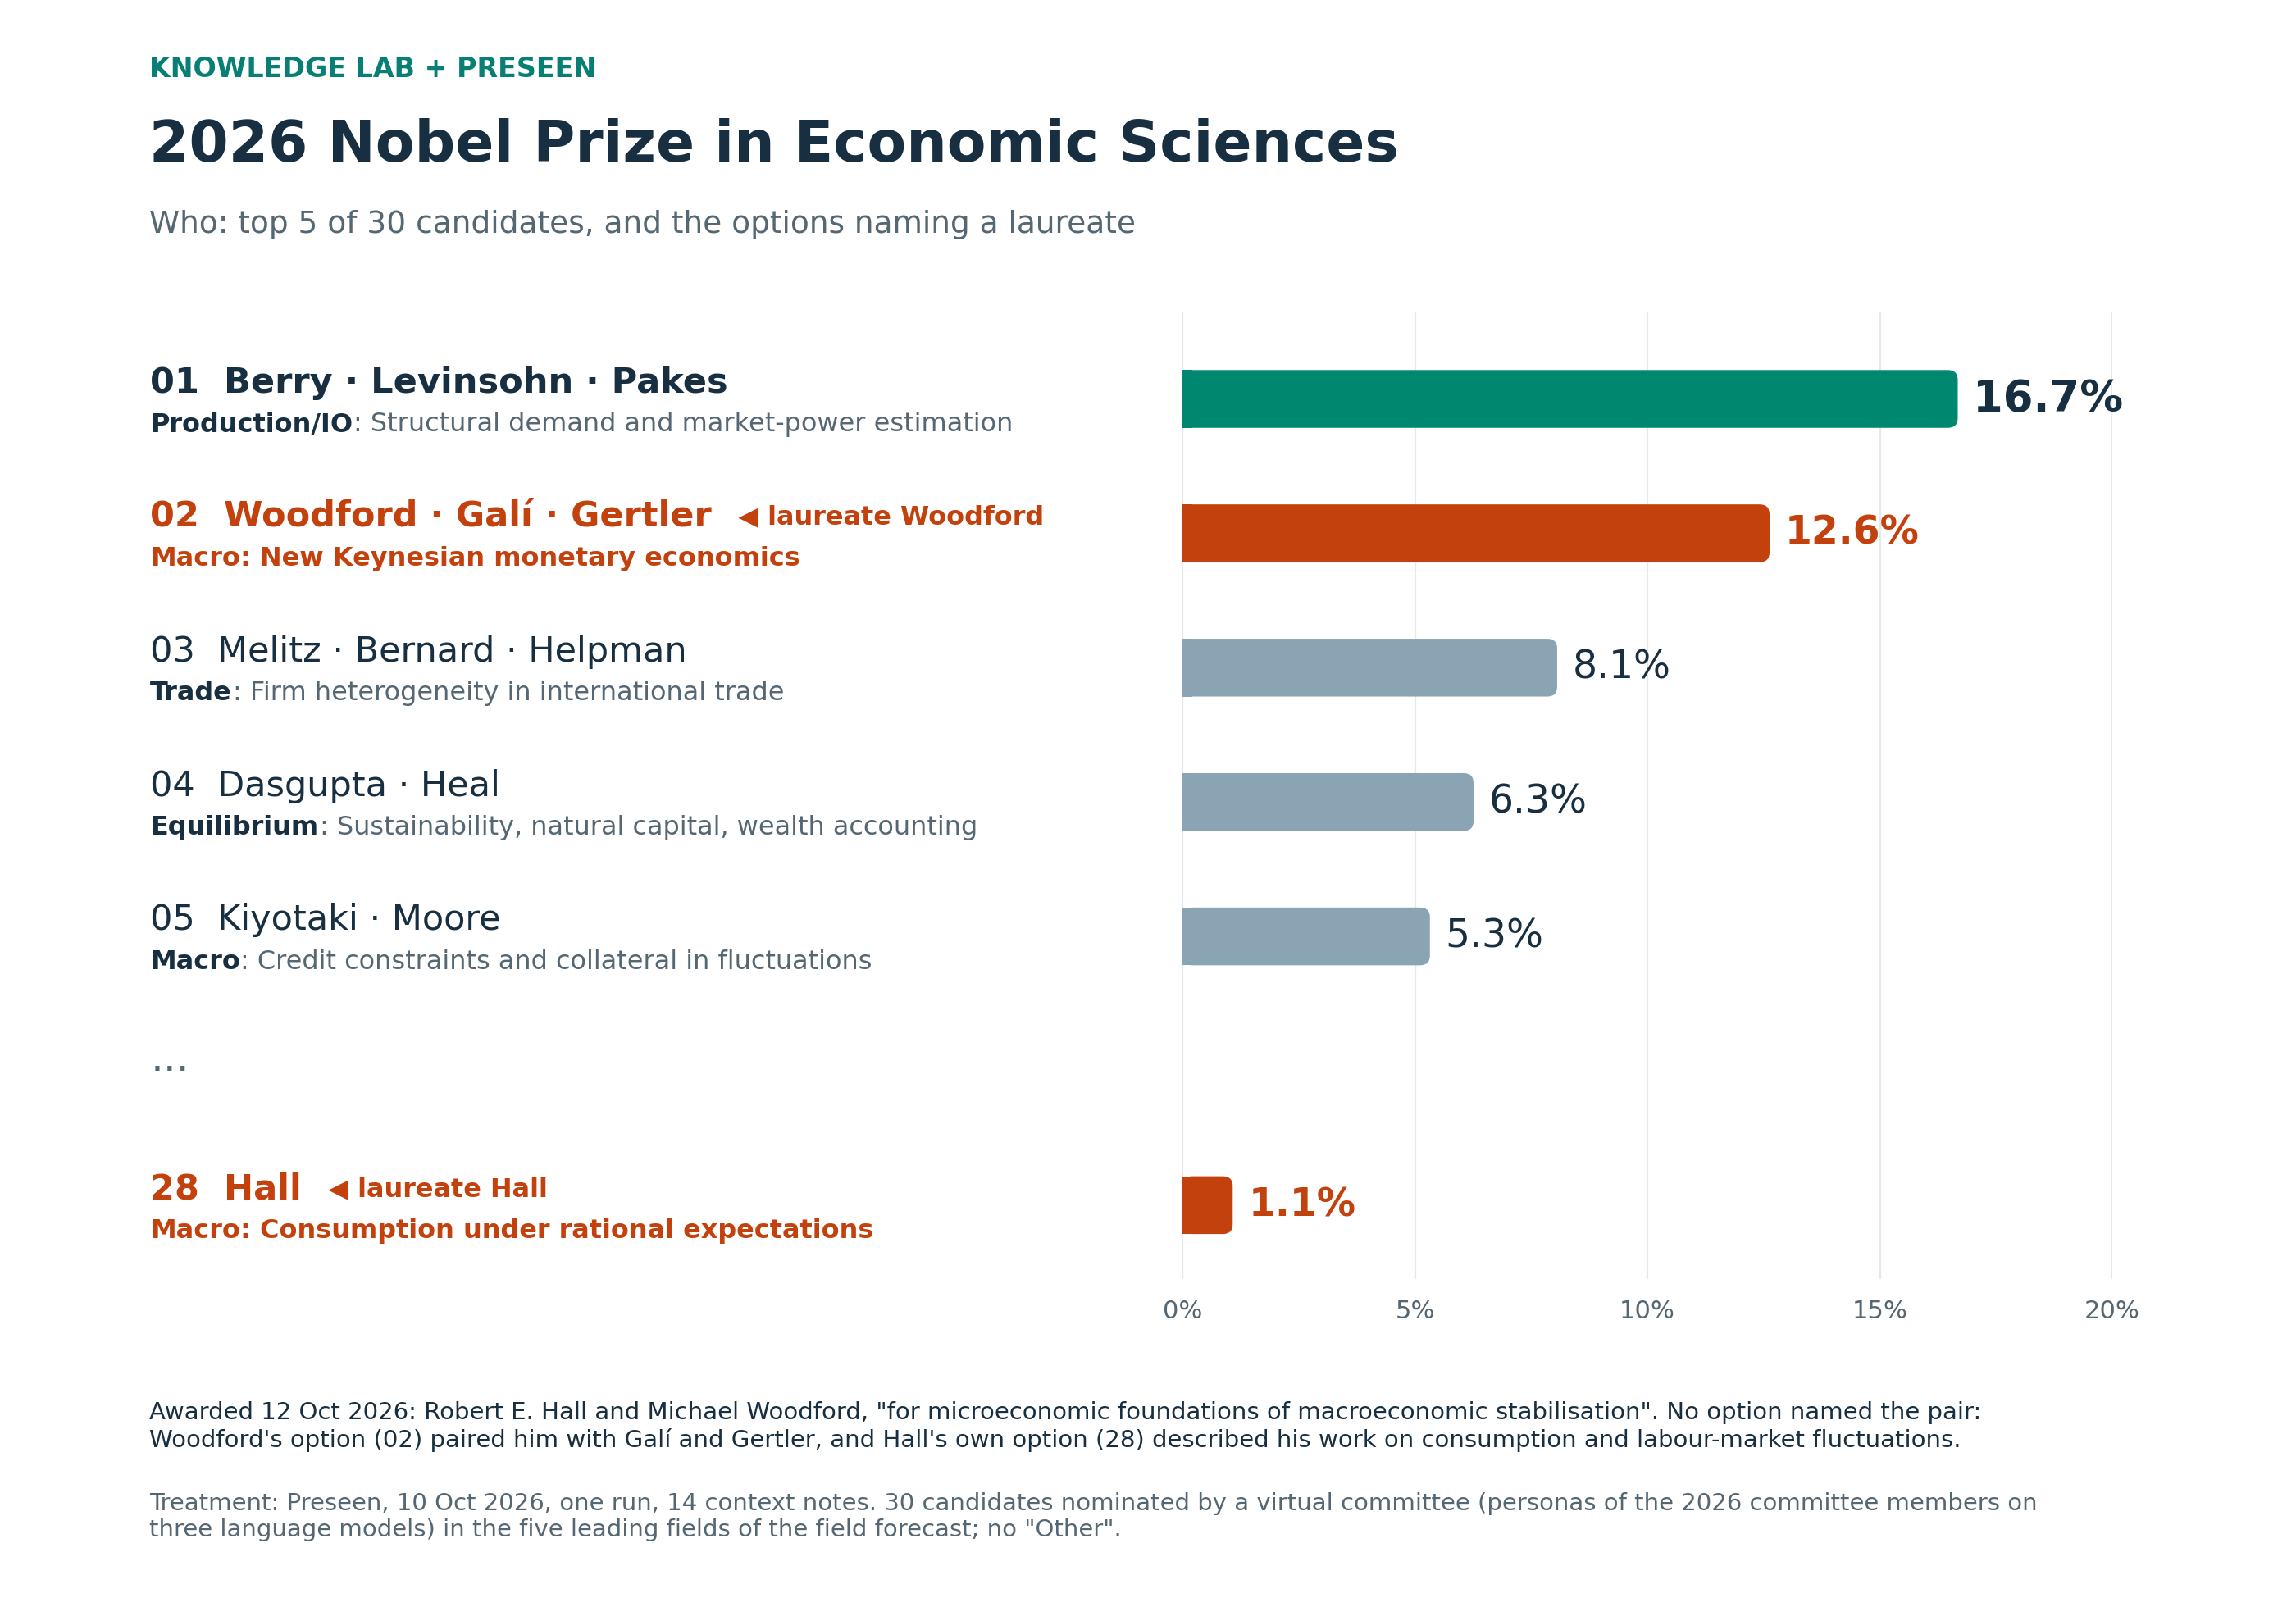
\includegraphics[width=0.85\textwidth]{economics_2026_people_top5_vs_award.png}
\caption{People forecast, treatment: the top five of 30 and the options naming a laureate
(\ttc{docs/nobel2026/make_econ_figures.py}).}
\end{figure}

\paragraph{Reading.} This time one of the two laureates was inside Preseen's top 5, but in a different combination:
\#2 (12.6\,\%), Woodford + Galí + Gertler --- Macro: New Keynesian monetary economics. Michael Woodford, and
macroeconomic stabilisation as the prize-winning contribution, were a near miss. The two-stage design (field
prediction, then candidate prediction within the top fields, built with Arna) had already put Macro at the top
(16.9\,\%). What we missed was the combination: Robert Hall did not appear in any of our top-5 configurations, and the
committee paired Woodford with him rather than with Galí and Gertler.

\begin{table}[htbp]
\small
\begin{tabularx}{\textwidth}{@{}P{30mm}LL@{}}
\toprule
Stage & Michael Woodford & Robert E. Hall \\
\midrule
Field question & Macro first in both arms (treatment 16.9\,\%, control 17.7\,\%; first experiment 16.8\,\% first and 14.5\,\% second) & same field \\
Virtual committee (165 macro nominations) & named in 29, by all 11 personas on all three models; his candidate (with Galí, Gertler) first in Macro, score 12.1 of 15 & named in 15, by 10 of 11 personas, mostly at rank 4--5 and alone (consumption under rational expectations, labour-market fluctuations): sixth of 26, score 2.3; once with Shimer and Hagedorn (24th) \\
Pool of 30 & Macro option 1 & Macro option 6, alone \\
People question & treatment 12.6\,\% (2nd), control 17.3\,\% (2nd) & treatment 1.1\,\% (28th), control 1.9\,\% (15th) \\
\bottomrule
\end{tabularx}
\caption{Where the laureates stood at each stage. No ballot named the two together.}
\end{table}

\noindent The treatment's reservations about Hall were, verbatim, ``Two separate strands make the motivation less
compact; consumption and expectations overlap; advanced age'' (83 by the birth year in the notes; 6 of 99 earlier
laureates were 80 or older). The committee's reasoning had named closeness to the Friedman (1976) and Modigliani (1985)
prizes.

\paragraph{Resolution and scores.} The motivation is about macroeconomic stabilisation (JEL E), so the field question
resolves to Macro. In the people question each of option 2 (Woodford's half: the New Keynesian
framework of nominal rigidities and welfare-based monetary policy analysis) and Hall's option (part of Hall's half)
names one laureate; under the tie rule option 2 is the nearer match. We report it as a near miss, a partial match:
the awarded pair was not an option. Log scores (ln $p$): field question treatment $-1.78$, control $-1.73$, uniform
$-2.64$; people question read as option 2: treatment $-2.07$, control $-1.76$, uniform $-3.40$. Both arms beat uniform at
both stages; the control a little more, because it put more on Macro and on the New Keynesian option.

\paragraph{What it shows about the design.} The virtual committee saw both halves of the prize, but as two separate
contributions; the real committee joined a demand-side and a supply-side line of work under one motivation. Options
built one contribution at a time (the integration merges nominations of the \emph{same} contribution) can show such a
pairing only if a ballot proposes it.
%======================================================================================================================
\part{Results}\label{part:results}
%======================================================================================================================

\section{The science prizes}\label{sec:res-science}

\subsection{Physiology or Medicine (awarded 5 October)}

\textbf{Award:} Karl Deisseroth, Peter Hegemann and Georg Nagel, ``for their discoveries concerning light-gated ion
channels and optogenetics''. The question (12 discoveries + Other, 1--2 October) had optogenetics as option 2 with
Deisseroth, Hegemann and Miesenböck; options are matched by discovery, so it is the awarded option.

\begin{table}[htbp]
\footnotesize
\begin{tabularx}{\textwidth}{@{}P{38mm}rrrLrrr@{}}
\toprule
Condition & Runs & Optogenetics & Rank & Leading option & GLP-1 & Other & ln $p$ \\
\midrule
Control & 5 & 5.5 & 6 & GLP-1, 20.3 & 20.3 & 31.0 & $-2.89$ \\
Cards as context & 3 & 6.8 & 3 & GLP-1, 19.6 & 19.6 & 30.4 & $-2.68$ \\
Cards as one main source & 1 & 7.4 & 4 & orexin, 11.7 & 11.0 & 34.0 & $-2.61$ \\
\textbf{Cards as the main evidence} & 1 & \textbf{7.9} & \textbf{1} & optogenetics, 7.9 & 3.0 & 40.0 & $-2.54$ \\
\bottomrule
\end{tabularx}
\caption{Medicine (\%). Log score of the mean probability of the awarded option; a uniform forecast over 13 options
scores $\ln(1/13)=-2.56$. Runs: \ttc{experiment/preseen_cards_main/results/medicine/runs_long.csv}.}
\end{table}

\noindent The more weight the forecaster was told to give the cards, the higher optogenetics ranked (sixth without
them, first as the main evidence) and the lower the award favourite GLP-1 (20.3\,\% to 3.0\,\%), while ``Other'' grew
from 31\,\% to 40\,\%. Only the main-evidence condition beat a uniform forecast.

\begin{figure}[htbp]
\centering
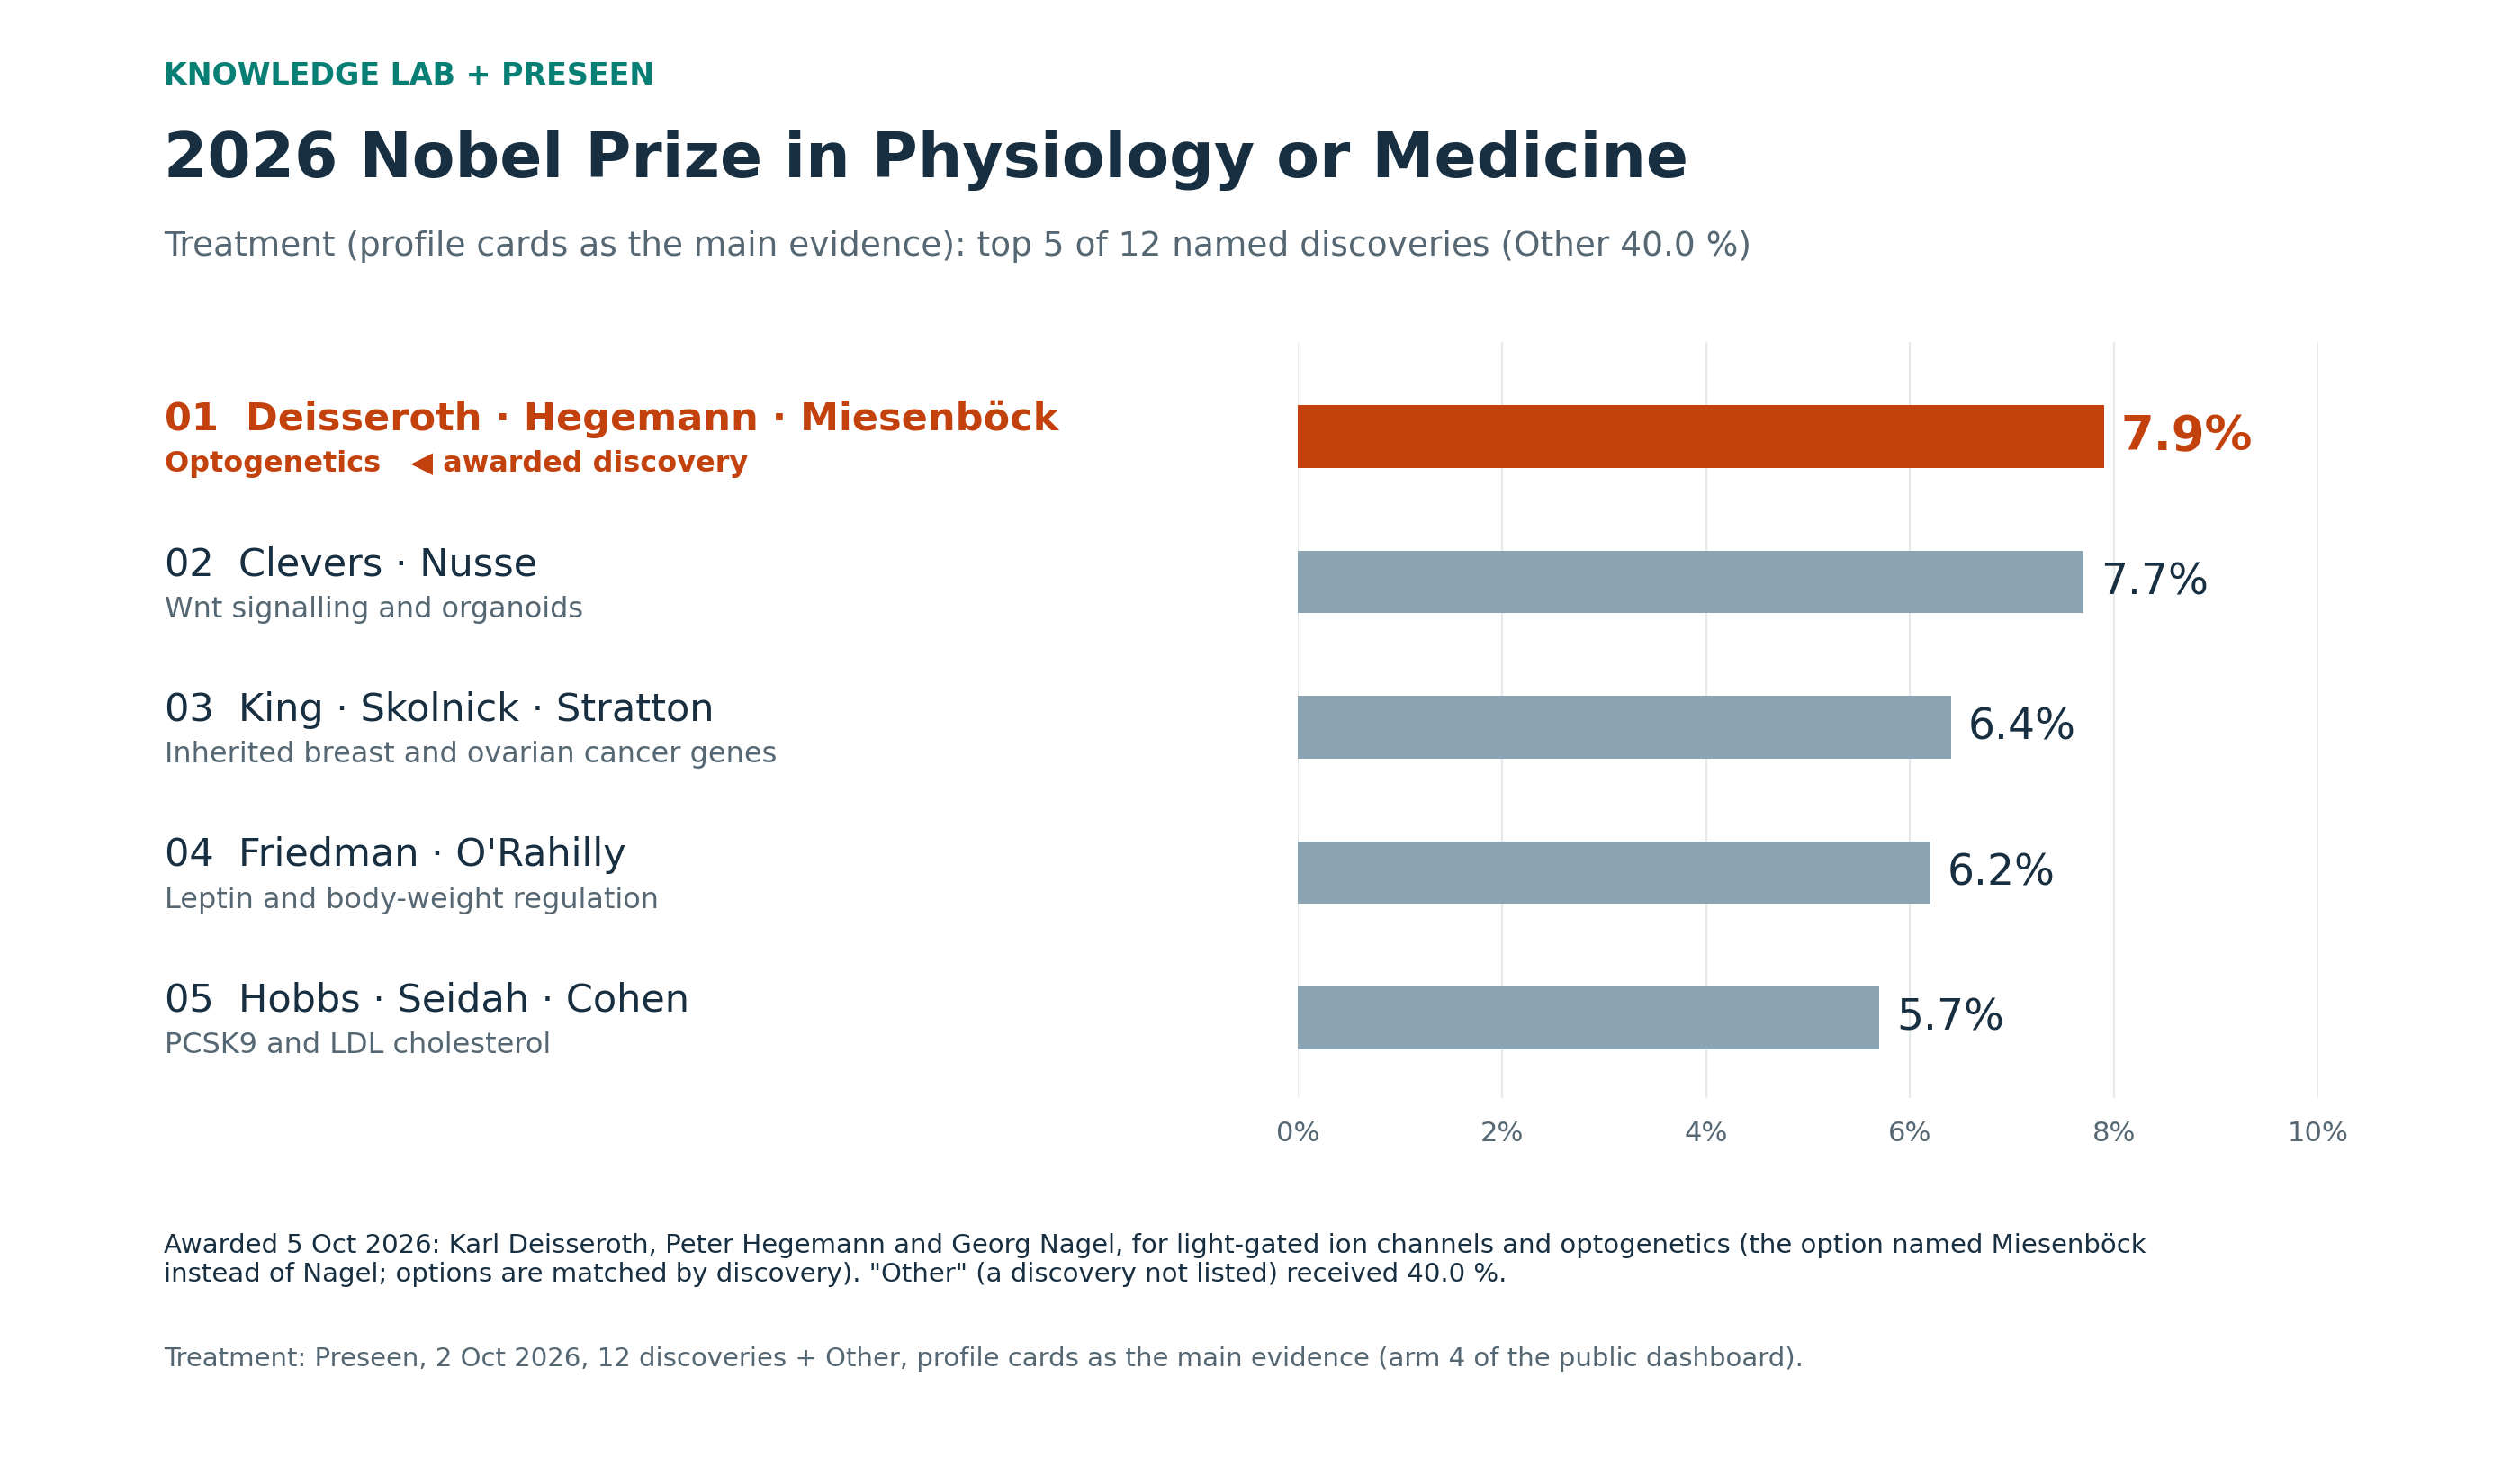
\includegraphics[width=0.78\textwidth]{medicine_2026_top5_vs_award.png}
\caption{Medicine, cards as the main evidence (2 October).}
\end{figure}

\subsection{Physics (awarded 6 October)}

\textbf{Award:} Francis Halzen alone, ``for decisive contributions to the IceCube Neutrino Observatory and the discovery
of high-energy neutrinos of astrophysical origin''. Neutrino astronomy was option 7 of the 12 and option 14 of the
30-option list (named Halzen, Karle, Kurahashi Neilson).

\begin{table}[htbp]
\footnotesize
\begin{tabularx}{\textwidth}{@{}P{24mm}P{36mm}rrrLr@{}}
\toprule
Question & Condition & Runs & Neutrino astronomy & Rank & Leading option & ln $p$ \\
\midrule
12 + Other (1--2 Oct) & control & 5 & 3.7 & 9 & optical lattice clocks, 14.7 & $-3.29$ \\
 & cards as context & 3 & 4.1 & 9 & optical lattice clocks, 15.4 & $-3.20$ \\
 & cards as one main source & 1 & 3.0 & 9 & quantum simulation, 12.8 & $-3.50$ \\
 & cards as the main evidence & 1 & 2.1 & 11 & quantum simulation, 13.3 & $-3.86$ \\
30 discoveries (5 Oct) & control & 1 & 3.1 & 11 & optical lattice clocks, 13.7 & $-3.47$ \\
 & \textbf{cards as the main evidence} & 1 & 3.5 & 14 & quantum simulation, 8.7 & $-3.35$ \\
\bottomrule
\end{tabularx}
\caption{Physics (\%). Uniform: $-2.56$ (13 options), $-3.40$ (30 options). The 5-option run did not contain the
awarded discovery and is annulled.}
\end{table}

\noindent The forecasters discounted neutrino astronomy for collaboration-scale attribution (IceCube papers are signed
by hundreds) and the neutrino prizes of 2002 and 2015. The committee answered the attribution question by giving the
prize to one person; two of the four committee nominations of the discovery had named Halzen alone, and the
astroparticle persona of all three models ranked him first. The v2 lineup rule (Section~\ref{sec:convergence}) would
have shown Halzen alone.

\subsection{Chemistry (awarded 7 October)}

\textbf{Award:} Henri B. Kagan and Kenso Soai, ``for the discovery of non-linear effects and autocatalysis in asymmetric
organic synthesis''. No committee nomination named them or the discovery; Soai appeared once in the convergence evidence
(2021 Nobel Symposium ``Chiral Matters'', filed under physics, one evidence family where two were needed); Preseen's own
list of 30 had Jacobsen's asymmetric epoxidation (2.5\,\%) as the nearest option. All five 30-option forecasts of 6
October are therefore annulled; only the 12 + Other question of 1--2 October can be scored, through ``Other'':

\begin{center}
\small
\begin{tabular}{@{}lrrr@{}}
\toprule
Condition & Runs & Other & ln $p$ \\
\midrule
Control & 5 & 33.6 (32.0--34.6) & $-1.09$ \\
Cards as context & 3 & 33.1 (32.1--34.4) & $-1.10$ \\
Cards as one main source & 1 & 37.5 & $-0.98$ \\
Cards as the main evidence & 1 & 38.0 & $-0.97$ \\
\bottomrule
\end{tabular}
\end{center}

\noindent The 30-option chemistry forecasts (annulled) show how far the conditions move a forecast: rank correlation
with the control 0.88 (cards as context), 0.71 (one main source), 0.32 (main evidence). Sequencing-by-synthesis went
from 17.3\,\% (control) to 22.9\,\% (context), 12.5\,\% (one main source, the README's main result) and 3.5\,\% (main
evidence); theoretical options without patents fell to 1.4\,\% when the main-evidence forecaster weighted patents; the
demographic factors stayed within 0.94--1.10.

\section{Economic Sciences (awarded 12 October)}

See Section~\ref{sec:econ-outcome}: Macro first in both field arms; Woodford in the second of 30 options (12.6\,\%
treatment, 17.3\,\% control) with Galí and Gertler; Hall alone 28th (treatment) and 15th (control).

\section{Scores across the four prizes}\label{sec:scores}

\begin{table}[htbp]
\small
\begin{tabularx}{\textwidth}{@{}lLrrrr@{}}
\toprule
Prize & Question (awarded option) & Control & Best condition & Main condition & Uniform \\
\midrule
Medicine & 12 + Other (optogenetics) & $-2.89$ & $-2.54$ (main evidence) & $-2.54$ & $-2.56$ \\
Physics & 12 + Other (neutrino astronomy) & $-3.29$ & $-3.20$ (cards as context) & $-3.86$ & $-2.56$ \\
Physics & 30 options (neutrino astronomy) & $-3.47$ & $-3.35$ (main evidence) & $-3.35$ & $-3.40$ \\
Chemistry & 12 + Other (Other) & $-1.09$ & $-0.97$ (main evidence) & $-0.97$ & $-2.56$ \\
Economics & 14 fields (Macro) & $-1.73$ & $-1.78$ (treatment) & $-1.78$ & $-2.64$ \\
Economics & 30 candidates (option 2, partial match) & $-1.76$ & $-2.07$ (treatment) & $-2.07$ & $-3.40$ \\
\bottomrule
\end{tabularx}
\caption{Log scores $\ln p$ of the awarded option (higher is better), from the mean probability over runs.
Chemistry's 30-option forecasts are annulled. The economics people question is scored under the reading of
Section~\ref{sec:econ-outcome}.}
\end{table}

\section{What we learned}\label{sec:lessons}

\begin{itemize}
\item \textbf{The context changes the forecast far more than the names on an option.} With \code{consider}-only cards
  the forecaster moved options by 0.53--0.72 times its own run-to-run noise (1 October) and used the cards ``as a
  secondary cross-check''; an \code{assume_true} instruction to use them as the main evidence moved options by 4.5--6.2
  times the noise (2 October) and collapsed the award favourites (GLP-1, optical lattice clocks, sequencing-by-synthesis).
\item \textbf{Profile cards favour academically cited careers.} Under ``main evidence'' the forecaster ranks options by
  the career impact of the named people. That helped optogenetics, but it pushed down inventions whose evidence sits in
  patents rather than papers; with a fixed weight on patents, theoretical discoveries without patents fell instead.
\item \textbf{Name the people the evidence supports, not three by default.} Physics went to one person; half of the
  committee's nominations of the discovery had said so.
\item \textbf{The pairing is part of the forecast.} Economics joined two lines of work under one motivation; our
  committee nominated both, separately. Options built one contribution at a time cannot express such a pairing unless a
  ballot proposes it.
\item \textbf{A list without ``Other'' cannot score a surprise.} The 30-option questions forecast which listed
  discovery wins, given that one does; the Chemistry award fell outside every list. The rule that an option the committee
  did not name needs two evidence families dropped the one signal we had.
\item \textbf{The two-stage design worked at the field level.} Macro, 20 years since its last award, was first in all
  four field runs except one control where it was second; candidates were then concentrated in the right field.
\end{itemize}
%======================================================================================================================
\part{User manual}\label{part:usage}
%======================================================================================================================

\section{Environment}\label{sec:env}

\subsection{Machine, Python, notebooks}

Everything runs on Midway3 (UChicago RCC). The Python environment is the \code{Curvature} conda env, called by path;
pandas and pyarrow need its own C++ runtime library:

\begin{Verbatim}
cd "/project/jevans/Dawoon/Nobel Prize"
export LD_LIBRARY_PATH=/project/jevans/Dawoon/env/Curvature/lib
PY=/project/jevans/Dawoon/env/Curvature/bin/python
NB="$PY -m jupyter nbconvert --to notebook --execute --inplace --ExecutePreprocessor.kernel_name=curvature"
\end{Verbatim}

\noindent The Jupyter kernel must be \code{curvature} (the default \code{python3} kernel is the system Anaconda without
DuckDB). Elsewhere: Python 3.12 with \file{requirements.txt} and a kernel of that name; then point the paths at the top
of \file{notebook/np_common.py} (\code{ROOT}, \code{SOS}, \code{OA_RAW}, \code{AUTHORSHIPS}, \ldots) to local copies of
the data.

\paragraph{Login node or compute node.} The login node caps a user at 8\,GiB of memory: name resolution, question
building, context notebooks, Preseen client calls and figure scripts run there; profiles and anything that scans the
large tables run as Slurm jobs (\file{jobs/*.sbatch}: \code{-p jevans -A pi-jevans --qos=jevans}, 8 cores, 96\,GB in
\file{author_profile.sbatch}, which executes a copy of the notebook into the person's output folder). Compute nodes have
internet access (OpenAlex API).

\paragraph{Shell scripts that run for an hour} (the \code{run_*.sh} scripts that create questions, add notes, run and
poll) are started in \code{tmux} or with \code{nohup} so that they survive a closed terminal; their logs are the
\code{*.out} files beside them. Never edit a shell script while a running bash is executing it (bash reads scripts
incrementally; one table step broke this way).

\subsection{API keys}\label{sec:keys}

Keys reach the code only as environment variables, read with \code{os.environ[...]} inside Python at the moment of a
request and sent only in headers. Nothing prints, logs or writes a key; no key is ever typed on a command line or put
in a file of the repository.

\begin{center}
\small
\begin{tabular}{@{}ll@{}}
\toprule
Variable & Service \\
\midrule
\code{PRESEEN_API_KEY} & Preseen \\
\code{COMMITTEE_ANTHROPIC_API_KEY} & Anthropic (never \code{ANTHROPIC_API_KEY}, which stays unset) \\
\code{OPENAI_API_KEY} & OpenAI \\
\code{GEMINI_API_KEY} & Google Gemini \\
\bottomrule
\end{tabular}
\end{center}

\begin{Verbatim}
$PY experiment/preseen/check_keys.py              # set/missing + HTTP status of one free GET per API, model ids
$PY experiment/preseen/check_keys.py --no-models  # status table only
\end{Verbatim}

\noindent A key works when its GET returns 200. Slurm jobs submitted with \code{--export=ALL} inherit the environment,
so the scripts that submit jobs (\file{submit_profiles.py}) remove the key variables first; do the same by hand:
\begin{Verbatim}
env -u PRESEEN_API_KEY -u COMMITTEE_ANTHROPIC_API_KEY -u OPENAI_API_KEY -u GEMINI_API_KEY sbatch ...
\end{Verbatim}
\noindent When an
editor's shell holds old keys (it happened on 10 October: 401 for Anthropic and OpenAI), run the paid steps from a
terminal that has the current keys (the Econ \file{run_all.sh} checks all three keys first).

\subsection{LaTeX}

\begin{Verbatim}
export PATH=/software/texlive-2023/bin/x86_64-linux:$PATH       # the texlive/2023 module has no pdflatex format
export TEXMFVAR=/scratch/midway3/$USER/texmf-var2023b            # home is near its quota
mkdir -p build
for i in 1 2 3; do pdflatex -interaction=nonstopmode -output-directory build FILE.tex > build/run$i.log; done
\end{Verbatim}

\noindent Do not redirect pdflatex's output to \file{<job>.out}: hyperref writes its outline to that file.

\section{Recipes: research profiles}\label{sec:use-profiles}

\begin{Verbatim}
$PY pipeline/profile_person.py "Geoffrey Hinton" --wait                 # resolve, run, print dashboard and record paths
$PY pipeline/profile_person.py "Geoffrey Hinton" --dry-run              # only the candidates and the choice
$PY pipeline/profile_person.py "Geoffrey Hinton" --affiliation "University of Toronto"
$PY pipeline/profile_person.py "Geoffrey Hinton" --pick 1               # rank 1 of the printed candidate table
$PY pipeline/profile_person.py --author-id "A5108093963;A5110248343" --wait
$PY pipeline/profile_person.py --names-file people.txt --wait           # one "name[<TAB>affiliation]" per line
$PY pipeline/profile_person.py "Jonghoon Kim" --author-id A5100409369 \
    --works-file Data/work_lists/A5100409369.txt --year-max 2022        # namesake-merged record: keep listed works only
\end{Verbatim}

\noindent Exit status: 0 when every query was profiled (or resolved with \code{--dry-run}, or submitted without
\code{--wait}); 2 when a query needs a choice (the candidate table is printed and nothing is submitted); 1 on any other
failure.

\begin{longtable}{@{}P{42mm}P{119mm}@{}}
\toprule
Option & Meaning \\
\midrule
\endhead
\code{name} & first + last name; titles, \code{Jr.}, parentheses and \code{née} are removed; a single name needs \code{--author-id} \\
\code{--affiliation TEXT} & candidates at this institution rank first \\
\code{--orcid ID} & decides when a candidate carries it \\
\code{--author-id A...;A...} & skip the search \\
\code{--pick N} & take rank $N$ of the printed table \\
\code{--dominance X} & automatic choice needs X times the citations of the next candidate (default 3) \\
\code{--no-merge} & do not add same-name fragments \\
\code{--works-file FILE} & only these works of the record (one OpenAlex work id per line) \\
\code{--no-api} & snapshot candidates only \\
\code{--label-year}, \code{--label-field} & first two parts of the file names (default: prize year and field, else \code{NA}) \\
\code{--year-max YEAR} & last publication / grant year (default 2021) \\
\code{--titles api|<parquet>|''} & titles from the OpenAlex API (default), a shared table, or a scan of the raw works \\
\code{--names-file FILE} & batch of names; per-person options cannot be combined with it \\
\code{--dry-run}, \code{--wait}, \code{--local} & resolve only; wait for the job; run in the current allocation \\
\code{--mem}, \code{--cpus} & Slurm resources (default 64G, 8) \\
\bottomrule
\caption{Options of \ttc{pipeline/profile_person.py}.}
\end{longtable}

\begin{longtable}{@{}P{40mm}P{26mm}P{91mm}@{}}
\toprule
Variable & Default & Meaning \\
\midrule
\endhead
\code{NP_AUTHOR_ID} & \code{A5067184382} & OpenAlex author id \\
\code{NP_EXTRA_AUTHOR_IDS} & --- & further ids of the same person, \code{;}-separated \\
\code{NP_WORKS_FILE} & --- & work list \\
\code{NP_YEAR_MAX} & 2021 & last publication / grant year \\
\code{NP_ID_CHECK} & \code{auto} & author id check: \code{auto} or \code{off} \\
\code{NP_NAME_SEARCH} & \code{always} & PatentsView name search: \code{always}, \code{auto}, \code{off} \\
\code{NP_VERIFY_PQRS} & 1 & check pqrs inventor ids like name-search ids \\
\code{NP_PATENT_FILTER} & 1 & leave out a selected inventor id's namesake patents \\
\code{NP_FETCH_TITLES}, \code{NP_TITLES_TABLE} & 0, --- & add work titles; their source \\
\code{NP_NOBEL_LOOKUP} & \code{auto} & prize lookup: \code{auto}, \code{ids}, \code{off} \\
\code{NP_PRIZE_YEAR}, \code{NP_PRIZE_FIELD} & --- & override the file-name labels \\
\code{NP_QUERY}, \code{NP_RESOLUTION} & --- & the typed name and the choice, written into the record \\
\bottomrule
\caption{Environment variables of \ttc{notebook/author_profile.ipynb}.}
\label{tab:np-env}
\end{longtable}

\paragraph{Direct notebook run and batches.}
\begin{Verbatim}
sbatch --export=ALL,NP_AUTHOR_ID=A5108093963,NP_EXTRA_AUTHOR_IDS=A5110248343,NP_FETCH_TITLES=1,NP_TITLES_TABLE=api \
       jobs/author_profile.sbatch
# laureate batch: PrizeAtlas crawl (login node, internet), pre-pass, array of profiles, aggregate
$NB notebook/prizeatlas_crawl.ipynb                                  # -> Data/prizeatlas/
sbatch jobs/prizeatlas_prepass.sbatch                                # -> output/batch_prizeatlas/targets.tsv, title caches
sbatch --dependency=afterany:<prepass job> jobs/prizeatlas_dashboards.sbatch   # 20 array tasks; reruns skip done ids
sbatch jobs/nobel_laureate_papers.sbatch                             # laureate aggregate dashboard
\end{Verbatim}

\noindent \textbf{Shared caches.} The first job after a change of the \emph{Science of Science} source tables rebuilds the
shared percentile caches in \file{cache/}. Run \emph{one} job first and the rest after it: on 1 October 93 parallel jobs
collided while rebuilding them, and on 5 October 59 of 66 failed and left 228\,GB of temporary files.

\section{Recipes: a science forecast with 12 discoveries + Other}\label{sec:use-science}

Run from \file{experiment/preseen/}. Paid steps (LLM calls, Preseen runs) need the user's approval first.

\begin{Verbatim}
cd "/project/jevans/Dawoon/Nobel Prize/experiment/preseen"
# 1. committee (paid: about $7 for 66 cells)
$PY committee.py prompt --field medicine --persona 0     # print the exact prompt (free)
$PY committee.py test                                    # one persona on each model (3 calls)
$PY committee.py estimate                                # cost of all committees from the test usage
$PY committee.py run --fields medicine physics chemistry --workers 2
$PY committee.py collect --field medicine                # raw/ -> ballots.jsonl (run also collects)
# 2. aggregation and review: edit committee/<field>/merges.yaml (each entry with a reason), then
$PY committee.py aggregate --field medicine              # -> candidates.json, clusters.json, review.md
$PY check_living.py                                      # Wikidata screen -> committee/<field>/living_check.csv
# 3. question
$PY build_question.py                                    # -> questions/<field>.json
# 4. people and profiles
$PY dryrun_fast.py --fields medicine physics chemistry   # one-scan resolver dry run -> people/<field>_dryrun_fast.log
$PY people.py identity --field medicine --log medicine_dryrun_fast.log   # the dry-run log; + people/<field>_choices.yaml
$PY submit_profiles.py                                   # one Slurm job per id set; keys stripped; reuses finished profiles
# 5. cards
$PY build_cards.py reference                             # laureate reference at prize time (2000-2025)
$PY build_cards.py cards --field medicine                # cards/<field>/00_definitions.md + one card per person
$PY build_cards.py check A5108093963                     # headline metrics of one profile vs its record
# 6. Preseen (paid; remote state). One EXP_DIR and one tag per field.
export EXP_DIR=preseen_exp/medicine; TAG=nobel26-med
$PY nobel_preseen_exp.py --tag $TAG create --question questions/medicine.json --arms control treat
$PY nobel_preseen_exp.py --tag $TAG run --arms control --reps 1          # first look, before any context exists
$PY nobel_preseen_exp.py --tag $TAG add-context --arm treat --cards cards_v1/medicine/
$PY nobel_preseen_exp.py --tag $TAG run --arms control treat --reps 3
$PY nobel_preseen_exp.py --tag $TAG poll --wait && $PY nobel_preseen_exp.py --tag $TAG table
# 7. analysis
$PY analyze.py field --field medicine && $PY analyze.py pooled
$PY build_dashboard.py
# 8. after the announcement
$PY analyze.py score --field medicine --option 2         # option number of the awarded discovery (13 = Other)
\end{Verbatim}

\paragraph{Conditions on the same question} (2 October). From \file{experiment/preseen_cards_main/} and
\file{preseen_cards_balanced/}, inside tmux:
\begin{Verbatim}
cd ../preseen_cards_main && ./run_field.sh medicine nobel26-med-main
#   create --arms control treat; add-context instruction/ (assume_true); add-context cards/medicine/ (consider);
#   run --reps 1; poll --wait; table
cd ../preseen_cards_balanced && ./run_field.sh medicine nobel26-med-bal     # treat arm only
cd ../preseen_cards_main
$PY analyze_main.py field --field medicine && $PY analyze_main.py pooled
$PY analyze_main.py score --field medicine --option 2
$PY build_dashboard2.py --fragment results/dashboard2_fragment.html
$PY ../build_dashboard_all.py                            # -> experiment/dashboard_all.html (Pages index.html on main)
\end{Verbatim}

\section{Recipes: 30-option lists, new cards and the later science runs}\label{sec:use-conv}

\paragraph{Option lists.}
\begin{Verbatim}
cd "/project/jevans/Dawoon/Nobel Prize/experiment/convergence_2026"
$PY build_options.py [--fields physics chemistry] [--k 30] [--weight 1.0]   # also rebuilds at weight/2 and weight*2
#   reads ../preseen/committee/<field>/ (ballots, merges.yaml), ../../Data/convergence_2026.csv, decisions.yaml
#   writes results/options_<field>.json|csv, results/review_<field>.md
cd ../convergence_2026_v2
$PY build_options_v2.py [--fields medicine physics chemistry] [--k 30] [--weight 1.0]   # v2 lineups
$PY compare_v1_v2.py                                    # results/compare_<field>.csv, compare.md, results/v1_rule/
\end{Verbatim}

\paragraph{Cards for the people of a new list} (the same steps in \file{convergence_2026/cards_pipeline.py} and
\file{convergence_2026_v2/cards_pipeline_v2.py}):
\begin{Verbatim}
$PY cards_pipeline_v2.py missing --write      # shown people without an identity -> people/<field>.txt
sbatch dryrun.sbatch                           # name search on a compute node -> people/<field>_dryrun.log
$PY cards_pipeline_v2.py identity              # -> people/<field>_identity.csv; hand picks in people/<field>_choices.yaml,
                                               #    record fixes in people/overrides.yaml
$PY cards_pipeline_v2.py living                # Wikidata check of every shown person -> people/living_check.csv
$PY cards_pipeline_v2.py submit --dry-run      # then without --dry-run: one Slurm profile per new id set
$PY cards_pipeline_v2.py submit --only "Name" --force [--no-name-search]   # rerun one profile
$PY cards_pipeline_v2.py cards                 # cards/<list>/<field>/ (K1)
$PY cards_pipeline_v2.py check                 # identity, profile and card for every shown person; exit 1 on a problem
\end{Verbatim}
Submit \emph{one} profile job first when the shared caches may be stale (Section~\ref{sec:use-profiles}).

\paragraph{Age-25 cards and blocks} (K2):
\begin{Verbatim}
cd ../convergence_2026
$PY cards_age25.py --field physics births      # births_physics.csv (+ laureate births); people/births_overrides.yaml
$PY cards_age25.py --field physics pools       # 80 most-cited works from age 25 on per person -> _work/pools_physics.json
#   defining works: LLM agents write picks per person -> cards_age25/defining_works_physics.yaml
$PY cards_age25.py --field physics reference   # age-25 laureate reference
$PY cards_age25.py --field physics cards       # cards_age25/physics/
$PY cards_age25.py --field physics check
$PY cards_age25.py --field physics blocks --question ../preseen_30_main_v2/questions/physics.json \
    --out ../preseen_30_main_v2/cards/physics [--no-lags]          # one option block per option
cd ../convergence_2026_v2                      # chemistry, v2 lists
$PY cards_age25_v2.py births --field chemistry && $PY cards_age25_v2.py pools --field chemistry
$PY cards_age25_v2.py merge-picks --field chemistry   # _work/picks/batch_*.yaml -> defining_works_chemistry.yaml
$PY cards_age25_v2.py reference --field chemistry && $PY cards_age25_v2.py cards --field chemistry
$PY cards_age25_v2.py check --field chemistry
\end{Verbatim}

\paragraph{Patents tied to the discovery} (K3):
\begin{Verbatim}
$PY patent_section.py pools --field chemistry   # cards_age25/_work/patent_pools/<slug>.json
#   LLM agents write cards_age25/_work/patent_picks/batch_*.yaml (up to 3 patents per person + n_related)
$PY patent_section.py merge --field chemistry   # -> cards_age25/patents_tied_chemistry.yaml (checked against the pools)
$PY patent_section.py apply --field chemistry   # inserts the section into cards/<list>/chemistry/ and the age-25 cards
\end{Verbatim}
The LLM-agent steps were run as parallel Claude subagents, one batch of people each. An agent that cannot read its
input files returns an empty pick list that looks complete: check every batch file before \code{merge-picks} or
\code{merge}.

\paragraph{Runs.} From the run folder, in tmux, with \code{PRESEEN_API_KEY} set:
\begin{Verbatim}
cd ../preseen_30_main_v2 && ./run_field.sh physics nobel26-phys-30-main-v2      # main arm (P3 + blocks)
./run_control.sh physics nobel26-phys-30-main-v2                                 # control arm, no notes
cd ../preseen_chem30_main
./run_list.sh v2 <tag>                          # main arm for one list (v1, v2, preseen)
./run_arm.sh v2 main3 <tag>                     # arms: main2, main3, demo, balanced, context
./run_control.sh v2 <tag>
python3 compare.py                              # results/compare.csv|md, write_up_<run>.md
python build_demographics.py                    # instruction_demo/00_6_demographics.md
\end{Verbatim}

\paragraph{Preseen-drafted list.}
\begin{Verbatim}
cd ../preseen_generated30 && EXP_DIR=chemistry $PY ../preseen/nobel_preseen_exp.py \
   normalize "Which discovery will the 2026 Nobel Prize in Chemistry be awarded for?" \
   --draft chemistry_draft.json --guidance "$(cat chemistry_guidance.txt)"      # -> chemistry/normalized.json
\end{Verbatim}
(The exact command line was not recorded; this is the client's syntax with the folder's inputs. Always set a fresh
\code{EXP_DIR}, or \file{preseen_exp/normalized.json} is overwritten.)

\paragraph{Handoff to Preseen} (\file{handoff/}; contexts and forecasts of the 1--2 October conditions kept apart):
\begin{Verbatim}
$PY handoff/build_handoff.py                    # regenerates handoff/context/, forecasts/, results.md
python handoff/post_notes.py --question <question id> --field medicine --condition cards_as_context [--dry-run]
#   --condition cards_as_context | cards_one_main_source | cards_main_evidence; --cards used|current;
#   --exclude <card id> ...; --only-options N ...   (posts notes only; never creates questions or runs)
\end{Verbatim}


\section{Recipes: the economics forecast}\label{sec:use-econ}

Run from \file{Econ/}; paid steps need the three model keys (Section~\ref{sec:keys}); Preseen steps need
\code{PRESEEN_API_KEY}. Every paid script keeps valid results and never asks again without \code{--force}; every call
is logged with tokens and cost in the step's \file{logs/calls.jsonl}.

\begin{Verbatim}
cd "/project/jevans/Dawoon/Nobel Prize/Econ"
# 0. prize record (free; nobelprize.org + Nobel Prize API)
$PY data/crawl_econ_prizes.py                    # --offline re-parses the newest raw files; exit 1 if a check fails
# 1. committee profiles (paid, ~$4.7)
$PY 01_committee/profiles.py roster
$PY 01_committee/profiles.py prompt --member john-hassler [--stage ask|merge]
$PY 01_committee/profiles.py estimate
$PY 01_committee/profiles.py test --member john-hassler
$PY 01_committee/profiles.py run [--members ...] [--providers ...] [--stages ask merge] [--workers 3]
$PY 01_committee/profiles.py merge [--members ...] [--force]
$PY 01_committee/profiles.py render && $PY 01_committee/profiles.py status
# 2. JEL coding (paid, ~$1.5) and the field analysis
$PY 02_fields/classify_jel.py prompt --batch 1
$PY 02_fields/classify_jel.py run [--providers ...] [--workers 2]   # then export + status automatically
$NB 02_fields/prize_history.ipynb                 # consensus, fields, sequence, gender, age; results/ and figures
# stage 1: field question
$NB 04_field_forecast/field_context_prompts.ipynb # context/00_1..00_9, questions/fields14.json, results/, record tables
cd 04_field_forecast
tmux -L econ new-session -d -s fields -c "$PWD" \
   'bash run_field.sh nobel26-econ-fields-nobel questions/fields14_nobel.json fields14_nobel > run_fields_nobel.out 2>&1'
#   run_field.sh [tag] [question] [state-subfolder]: create control+main, add the nine notes (assume_true),
#   run 1 rep each, poll --wait, table -> preseen_exp/<sub>/runs.csv and runs/*.json
cd ..
# 5. laureate ages (free)
$NB 05_laureates/laureate_history.ipynb           # results/, prompt/01_age_at_award.md
# stage 2a/2b: virtual committee and integration (paid, ~$11)
cd 06_candidates
$PY virtual_committee.py prompt --member john-hassler   # writes prompts/example_john-hassler__b1.md
$PY virtual_committee.py test --member john-hassler
$PY virtual_committee.py estimate
bash run_all.sh       # checks the three keys (HTTP 200), then nohup run_all_steps.sh > run_all.out:
                      #   run --workers 9; run --workers 6 (second pass); status; collect;
                      #   integrate; context; pool; estimate
$PY virtual_committee.py integrate --dry-run      # write the integration prompts without calling
$PY virtual_committee.py status
cd ..
# stage 2c: people question
cd 07_people_forecast
$PY check_living_econ.py                          # Wikidata -> living_check.csv; decide unclear rows in living_overrides.yaml
$PY make_people_nb.py                             # (re)generates people_candidate_prompts.ipynb
$NB people_candidate_prompts.ipynb                # context/ (14 notes), questions/people30.json
nohup bash run_people.sh nobel26-econ-people questions/people30.json people30 \
   > run_people.out 2>&1 &                        # refuses unless context/ has 14 notes and living_check.csv exists
\end{Verbatim}

\paragraph{Knobs.} \file{06_candidates/settings.yaml}: \code{fields} (14 entries with \code{name, slug, batch, jel,
prefixes, main_pct, pool, definition}; batch 1 = the five asked fields with pools 7/7/6/6/4, set by hand from the field
forecast), \code{batches_to_ask: [1]}, \code{committee} (\code{max_nominations} 5, \code{max_people} 3,
\code{max_key_works} 3, \code{max_rationale_sentences} 3, \code{borda_points}, \code{link_min_overlap} 0.15,
\code{json_retries} 1), \code{integrate} (provider \code{anthropic}, \code{json_retries} 2, \code{max_defining_works}
4, \code{workers} 5), \code{pool_total} 30. The people notebook's first cell: \code{POOL}, \code{MAX_WORKS} (4),
\code{ORDER} (\code{committee} or \code{alphabetical}), \code{SHOW_BORN}, \code{FIELD_PCT}, \code{PROVENANCE},
\code{AWARDED_OTHER_SINCE} (2000), \code{OTHERS_SHOWN} (5).

\paragraph{Things to know.}
\begin{itemize}
\item \code{integrate} records a sha256 stamp of its input ballots; \code{context}, \code{pool} and the people
  notebook refuse a stale integration. \code{pool} drops candidates with an empty lineup or a laureate or committee
  flag, but not deceased people; the people notebook removes them (\code{living_overrides.yaml}).
\item The client posts the \code{00_*} notes first and the others in a seeded random order (seed 2026), so the 14
  people-stage notes were not uploaded in name order. In the field stage all nine notes are \code{00_*}.
\item The generators of \file{field_context_prompts.ipynb} and \file{laureate_history.ipynb} were session scripts
  outside the repository; the notebooks are the source of truth. \file{make_people_nb.py} is in the repository.
\item Exact copies of what was uploaded on 10 October are kept in \file{04_field_forecast/uploaded_2026-10-10/} (the
  live \code{00_5} has the corrected 2022 ages).
\end{itemize}


\section{Recipes: after an announcement}\label{sec:use-after}

\begin{enumerate}
\item Fetch the award from the Nobel Prize API (no key), for example
  \url{https://api.nobelprize.org/2.1/nobelPrizes?nobelPrizeYear=2026&nobelPrizeCategory=eco}: laureates, shares
  (\code{portion}), motivation, affiliations, birth dates (recompute ages from the dates).
\item Decide which option the motivation resolves to under the question's own criteria (by discovery or contribution;
  the people need not match). Write down the reading when it is a partial match.
\item Score: \code{analyze.py score} / \code{analyze_main.py score} for the 12 + Other runs; for the other runs the log
  of the awarded option's probability from the run tables.
\item Figures: mark the awarded option in \file{docs/nobel2026/make_figures.py} (\code{awarded} rank, or
  \code{unlisted} for an award outside the list) or \file{make_econ_figures.py} (\code{LAUREATES}) and rerun; both write
  to \file{docs/nobel2026/} and \file{Data/Result/<Field>/}.
\item README: the field's collapsible section in the main \file{README.md} (summary line = award + the main forecast's
  standing), and the field's own README.
\item Commit on \code{preseen-nobel-2026}, merge into \code{main} (from a separate worktree of \code{main}), push both
  (Section~\ref{sec:versioned}).
\end{enumerate}
\section{Repository layout}\label{sec:layout}

\begin{Verbatim}
Nobel Prize/
  README.md                      public front page: the four forecasts against the awards (collapsible sections)
  requirements.txt, .gitignore
  pipeline/profile_person.py     name -> author id -> Slurm job -> dashboard + record
  notebook/                      author_profile.ipynb, nobel_laureate_papers.ipynb, prizeatlas_crawl.ipynb,
                                 chemistry2026_sleeping_beauty.ipynb, np_common.py (shared functions)
  jobs/                          Slurm runners (author_profile, prizeatlas_prepass, prizeatlas_dashboards,
                                 nobel_laureate_papers); logs/ (not versioned)
  docs/author_profiles.md        documentation of the profile pipeline; docs/example/hinton/ figures
  docs/nobel2026/                README figures, make_figures.py, make_econ_figures.py
  Data/                          prizeatlas/ (CSV), Li2019/, SciSciNet_Link_NobelLaureates.tsv, convergence_2026.csv,
                                 work_lists/, Result/ (forecast tables, Preseen reports, figures per field)
  experiment/
    preseen/                     1 Oct: committee, question, people, profiles, cards, runs, analysis, dashboard
    preseen_cards_main/          2 Oct: cards as the main evidence (+ analyze_main.py, build_dashboard2.py)
    preseen_cards_balanced/      2 Oct: cards as one main source
    build_dashboard_all.py       combined page of the four conditions (Pages index.html)
    convergence_2026/            5 Oct: 30-option lists (physics, chemistry), cards pipeline, age-25 cards
    convergence_2026_v2/         6 Oct: v2 lineups, medicine list, cards, patents tied to the discovery
    preseen_main_no_other/, preseen_30_no_other/, preseen_12_main_v2/, preseen_30_main_v2/, preseen_5_main_v2/
                                 5 Oct physics runs
    preseen_chem30_main/         6 Oct chemistry runs (five conditions, compare.md)
    preseen_generated30/         6 Oct: a list of 30 drafted by Preseen
  Econ/                          the economics pipeline (Part III); record/Record.tex
  handoff/                       contexts and forecasts of 1-2 Oct for Preseen
  manuscript/                    preseen_nobel2026_experiment.tex (1 Oct experiment), this document
  output/, cache/                profiles and shared caches (not versioned; tens of GB)
\end{Verbatim}

\section{What is versioned, and how to publish}\label{sec:versioned}

\begin{itemize}
\item \textbf{Versioned:} code, notebooks without outputs, READMEs, small tables (CSV), questions, context notes,
  cards, analysis tables, figures, Preseen report PDFs, LaTeX sources and PDFs.
\item \textbf{Not versioned} (\file{.gitignore}): \file{output/}, \file{cache/}, \file{jobs/logs/},
  \file{Data/prizeatlas/html/}, every \file{*.parquet}, Preseen client state (\file{experiment/**/preseen_exp/},
  \file{Econ/**/preseen_exp/}), raw committee responses (\file{committee/*/raw/}), run logs (\file{*.out}), title caches,
  key checkers and session helpers.
\item \textbf{Notebooks} are committed without outputs while the working copies keep theirs: stage a stripped blob
  (\code{git hash-object -w --stdin} on the stripped JSON, then \code{git update-index --cacheinfo}), so the working tree
  shows them as modified afterwards.
\item \textbf{No secrets, no ids:} scan the staged files for keys and for Preseen question and task ids before
  committing (the public LOGs were cleaned of ids on 3 October).
\item \textbf{Branches:} commit on \code{preseen-nobel-2026}; merge into \code{main} from a separate worktree that has
  \code{main} checked out (the project folder stays on the branch); push both. The GitHub web editor has been used on
  \code{main}: fetch and merge \code{origin/main} into the branch before the next push.
\end{itemize}

\section{Costs}\label{sec:costs}

\begin{center}
\small
\begin{tabularx}{\textwidth}{@{}lrL@{}}
\toprule
Item & USD & Note \\
\midrule
Science committee, 66 cells (1 Oct) & 7.12 & claude-opus-5-5 1.70, gpt-5.5 4.20, gemini-3.1-pro 1.22; tests about 0.33 \\
Econ committee profiles, 44 calls (9 Oct) & 4.66 & 33 descriptions + 11 merges \\
Econ JEL coding, 12 calls (9 Oct) & 1.52 & 4 batches $\times$ 3 models \\
Econ virtual committee, first run (archived) & 8.14 & 61 calls including tests \\
Econ virtual committee, second run & 8.30 & 33 cells, all valid at the first attempt \\
Econ integration & 2.33 & 5 Claude calls \\
Preseen questions, notes and runs & --- & Preseen credits; not reported by the API \\
Profiles, OpenAlex, Wikidata, ORCID & --- & cluster allocation; free APIs \\
\bottomrule
\end{tabularx}
\end{center}

\noindent Prices used for estimates (\file{config.yaml}, USD per million tokens, input / output):
\code{claude-opus-5-5} 4 / 20, \code{gpt-5.5-2026-04-23} 5 / 30, \code{gemini-3.1-pro-preview} 2 / 12.

\section{Traps and lessons}\label{sec:traps}

\begin{longtable}{@{}P{42mm}P{119mm}@{}}
\toprule
Problem & What to do \\
\midrule
\endhead
Reference-less papers have CD $=1$ & blank CD for documents without references; take percentiles among documents with references \\
Stale shared caches & after the \emph{Science of Science} sources change, run one profile job first; parallel jobs collide on the cache rebuild \\
OpenAlex namesake merges & check the identity table; use \code{--works-file}, age-25 windows, \code{people/<field>_choices.yaml} hand picks \\
PatentsView name lumping & inventor linking with clusters and evidence; read \file{inventor_link_patents.csv} for the cards' patents \\
Wikidata false matches & read every flagged row of the living check by hand; keep overrides in a file \\
Models name dead people & screen every shown person before a question is built (three in the science lists, two in economics) \\
Nobel API dates & the 2022 economics award is dated 2011; recompute ages from the dates and check against the prize year \\
\code{poll --wait} rewrites \code{state.json} & one \code{EXP_DIR} per arm group; never create a new arm in a folder a running poll uses \\
Editing a running shell script & do not; bash reads scripts incrementally \\
\code{pgrep -f} waits on itself & wait with \code{kill -0 PID} instead \\
\code{--export=ALL} copies keys into jobs & strip the key variables before \code{sbatch} \\
pandas empty object masks & \code{.astype(bool)} on \code{.map()} masks (an empty object mask selects columns) \\
A list without ``Other'' & conditional forecasts are annulled when the award is outside the list; keep a 12 + Other question as a scorable companion \\
Merged lineups & showing the top three names of every merged nomination invents lineups; show a lineup a nomination wrote (v2) \\
Agents denied file access & a workflow agent that cannot read returns empty picks that look completed; check every pick file \\
\bottomrule
\caption{Traps met while building and running the pipeline.}
\end{longtable}

\section{Limitations}\label{sec:limitations}

\begin{itemize}
\item The committees are simulations by three correlated language models, without web access; their nominations are
  not the views of real committee members, who were not consulted. Models trained on overlapping data share blind
  spots (no nomination named Kagan or Soai).
\item One forecasting system, mostly one run per condition: differences of a few percentage points between single runs
  are within noise (control runs differ by about 0.6--0.9 points per option).
\item The cards are bundles of many numbers and inherit the data problems of Section~\ref{sec:profile-caveats}; a
  placebo arm (the same cards with numbers shuffled across people) was planned and switched off.
\item Resolution by discovery or contribution needs judgment when a motivation is broader or narrower than an option
  (Medicine: Nagel instead of Miesenböck; Economics: a pair across two options).
\item The economics field rotation is a design assumption, not an estimated rule; the people pool covers the five
  leading fields only (69\,\% of the treatment's field probability).
\end{itemize}

\section*{References}
\addcontentsline{toc}{section}{References}
\begin{itemize}
\item Dolton, P.\ J.\ and Tol, R.\ S.\ J.\ (2026). The process and dynamics of the Nobel Memorial Prize in Economics,
  1969--2025. arXiv:2603.20767v1.
\item Fang, H.\ and Evans, J.\ (2025). Generalization and the rise of system-level creativity in science.
  arXiv:2510.03240 (the Foundation / Extension / Generalization decomposition).
\item Li, J., Yin, Y., Fortunato, S.\ and Wang, D.\ (2019). A dataset of publication records for Nobel laureates.
  \emph{Scientific Data} 6:33 (Harvard Dataverse doi:10.7910/DVN/6NJ5RN).
\item Marx, M.\ and Fuegi, A. Reliance on Science: patent-to-paper citations (CC BY 4.0).
\item OpenAlex (CC0); PatentsView (CC BY 4.0); PrizeAtlas (CC BY-SA 4.0, \url{https://prizeatlas.org}); SciSciNet
  laureate links; the Nobel Prize API 2.1 and \url{https://www.nobelprize.org}; Preseen (\url{https://preseen.com}).
\end{itemize}

\end{document}
